\documentclass[12pt,a4paper]{article}
%
\usepackage{amsmath}
\usepackage{amssymb}
\usepackage{amsthm}
\usepackage{graphicx}
%
\usepackage[colorlinks=true,allcolors=blue]{hyperref}
\usepackage[figurename={Figure}]{caption}
%\usepackage{url}
%
\newcommand{\mb}[1]{\mathbb{#1}}
\newcommand{\mf}[1]{\mathbf{#1}}
\newcommand{\G}{\mb{G}}
\newcommand{\R}{\mb{R}}
\newcommand{\Z}{\mb{Z}}
\newcommand{\abs}[1]{\left| #1 \right|}
\newcommand{\norm}[1]{\left\| #1 \right\|}
\newcommand{\isomorphic}{\simeq}
\newcommand{\To}{\rightarrow}
%
%
%\newcommand{\slidecite}[1]{\tiny{(#1)}\normalsize{}}
%\newcommand{\smallcite}[1]{\small{(#1)}\normalsize{}}

\newcommand{\Emph}[1]{\emph{\textcolor{blue}{#1}}}

\newcommand{\Cay}[1]{\operatorname{Cay}\left(#1\right)}
\newcommand{\Clique}[1]{\omega\left(#1\right)}
\newcommand{\diag}[1]{\operatorname{diag}\left(#1\right)}
\newcommand{\dual}[1]{\widetilde{#1}}
\newcommand{\support}[1]{\operatorname{supp}\left(#1\right)}
\newcommand{\weight}[1]{\operatorname{wt}\left(#1\right)}
\newcommand{\weightclass}[1]{\operatorname{wc}\left(#1\right)}

\newtheorem*{lemma}{Lemma}
\newtheorem{Lemma}{Lemma}
\newtheorem*{proposition}{Proposition}
\newtheorem{Proposition}{Proposition}
\newtheorem*{theorem}{Theorem}
\newtheorem{Theorem}{Theorem}
\newtheorem*{conjecture}{Conjecture}
\newtheorem{Conjecture}{Conjecture}
\newtheorem*{corollary}{Corollary}
\newtheorem{Corollary}[Lemma]{Corollary}
\newtheorem*{remark}{Remark}
\newtheorem{Remark}{Remark}
\newtheorem*{definition}{Definition}
\newtheorem{Definition}{Definition}
\newtheorem{Question}{Question}
\newtheorem{Questions}[Question]{Questions}
%
\newenvironment{proofof}[1]{\noindent\emph{Proof of #1.}}{\qed}

\title{INCOMPLETE DRAFT: \\
Classifying bent functions by their Cayley graphs}

\author{
Paul~Leopardi
%\thanks{Australian Government -- Bureau of Meteorology
\thanks{University of Melbourne, Australian Government -- Bureau of Meteorology
\protect\url{mailto:paul.leopardi@gmail.com}}
%\protect\texttt{mailto:paul.\-leopardi@anu.edu.au}}
}

\date{INCOMPLETE DRAFT: 30 April 2017}

\begin{document}

\maketitle

\begin{abstract}
%
%
\end{abstract}

\section{Introduction}
\label{sec-Introduction}
Binary bent functions are important combinatorial objects.
Besides the well-known application of bent functions and their generalizations to cryptography
\cite{Ada97} \cite[4.1-4.6]{Tok15bent},
bent functions have well-studied connections to Hadamard difference sets \cite{Dil74},
symmetric designs with the symmetric difference property \cite{DilS87block,Kan75symplectic},
projective two-weight codes \cite{DinD15class} and strongly regular graphs.

In two papers, Bernasconi and Codenotti \cite{BerC99}, and then Bernasconi, Codenotti and Vanderkam
\cite{BerCV01} explored some of the connections
between bent functions and strongly regular graphs.
While these papers established that the Cayley graph of a binary bent function (whose value at 0 is
0) is a strongly regular graph
with certain parameters, they leave open the question of which strongly regular graphs with these
parameters  be so obtained.
Kantor, in 1983 \cite{Kan83exponential}, showed that the number of non-isomorphic projective linear
two weight codes with certain parameters,
Hadamard difference sets, and symmetric designs with certain properties, grows at exponentially
with dimension.
This result suggests that the number of strongly regular graphs obtained as Cayley graphs of bent
functions also increases at least exponentially with dimension.

In a recent paper, the author found an example of two infinite series of bent functions whose
Cayley graphs have the same strongly regular parameters at each dimension,
but are not isomorphic if the dimension 8 or more \cite{Leo17Hurwitz}.

The goal of the current paper is to further explore the connections between bent functions, their
Cayley graphs, and related combinatorial objects,
and in particular to examine the relationship between various equivalence classes of bent
functions, in particular, the relationship between the extended affine
equivalence classes and equivalence classes defined by isomorphism of Cayley graphs.
As well as a theoretical study of bent functions of all dimensions, an empirical study is conducted
into bent functions of dimension at most 8,
using SageMath \cite{SageMath7517} and SageMathCloud \cite{SageMathCloud}.


% Two recent papers \cite{Leo14Constructions,Leo15Twin} describe and investigate two infinite sequences of bent functions and their Cayley graphs.
% The bent function $\sigma_m$ on $\Z_2^{2 m}$ is described in the first paper \cite{Leo14Constructions}, on
% generalizations of Williamson's construction for Hada\-mard matrices.
% The bent function $\tau_m$ on $\Z_2^{2 m}$ is described in the second paper \cite{Leo15Twin},
% which investigates some of the properties of the two sequences of bent functions.
% In this second paper it is shown that the bent functions $\sigma_m$ and $\tau_m$ both correspond to Hada\-mard difference sets with the same parameters
% \begin{align*}
% (v_m,k_m,\lambda_m,n_m) &= (4^m, 2^{2 m - 1} - 2^{m-1}, 2^{2 m - 2} - 2^{m-1}, 2^{2 m - 2}),
% \end{align*}
% and that their corresponding Cayley graphs are both strongly regular with the same parameters $(v_m,k_m,\lambda_m,\lambda_m)$.
%
% The main result of the current paper is the following.
% \begin{Theorem}\label{HR-non-imomorphic-theorem}
% The Cayley graphs of the bent functions $\sigma_m$ and $\tau_m$ are isomorphic only when $m=1, 2,$ or $3.$
% \end{Theorem}
%
The remainder of the paper is organized as follows.
% Section \ref{sec-Background} outlines some of the background of this investigation.
Section \ref{sec-Preliminaries} covers the concepts, definitions and known results used later in the paper.
Some of these concepts and definitions are novel, such as new notions of equivalence of bent
functions.
%Section \ref{sec-Equivalence} introduces various concepts of equivalence of bent functions.
Section \ref{sec-Results} contains the main theoretical results of the paper.
Section \ref{sec-Empirical} lists some of the properties of the equivalence classes of bent functions for dimension up to 8.
Section \ref{sec-Code} describes the SageMath and SageMathCloud code that has been used to obtain
and display these empirical results.
Section~\ref{sec-Discussion} puts these results in the context of questions that are still open.
%
% % \begin{frame}
% \subsection{Overview}
% %\begin{center}
% \begin{itemize}
% \item
% Key concepts.
%
% ~
%
% \item
% Equivalence.
%
% ~
%
% \item
% Some results.
%
% ~
%
% \item
% Observations for small dimensions.
%
% ~
%
% \item
% Some questions.
%
% ~
%
% \item
% SageMathCloud worksheet.
% \end{itemize}

%\end{center}
% \end{frame}

% \section{Background}\label{sec-Background}
% A recent paper of the author \cite{Leo14Constructions} describes a generalization of
% Williamson's construction for Hada\-mard matrices \cite{Wil44}
% using the real monomial representation of the basis elements of the Clifford algebras $\R_{m,m}$.
% In that paper, the following three conjectures appear:
%
% \begin{Conjecture}\label{conjecture-1}
% %
% For all $m \geqslant 0$ there is a permutation $\pi$ of the set of $4^m$ canonical basis matrices,
% that sends an amicable pair of basis matrices with disjoint support to an anti-amicable pair, and
%vice-versa.
% %
% \end{Conjecture}
%
% \begin{Conjecture}\label{conjecture-2}
% %
% For all $m \geqslant 0,$
% for the Clifford algebra $\R_{m,m},$ the subset of transversal graphs that are
% not self-edge-colour complementary
% can be arranged into a set of pairs of graphs with each member of the pair
% being edge-colour complementary to the other member.
% %
% \end{Conjecture}
%
% \begin{Conjecture}\label{conjecture-3}
% %
% For all $m \geqslant 0,$
% for the Clifford algebra $\R_{m,m},$ if a graph $T$ exists amongst the transversal graphs,
% then so does at least one graph with edge colours complementary to those of $T$.
% %
% \end{Conjecture}
%
% The author's subsequent paper on bent functions \cite{Leo15Twin}
% refines Conjecture~\ref{conjecture-1} into the following question.
% \begin{Question}
% \label{Question-1}
% Consider the sequence of edge-coloured graphs $\varDelta_m$ for $m \geqslant 1$,
% each with red subgraph $\varDelta_m[-1],$ and blue subgraph $\varDelta_m[1].$
% For which $m \geqslant 1$ is there an automorphism of $\varDelta_m$
% that swaps the subgraphs $\varDelta_m[-1]$ and $\varDelta_m[1]$?
% \end{Question}
%
% (The term \emph{transversal graph} and the definitions of $\varDelta_m$, $\varDelta_m[-1],$ and
%$\varDelta_m[1]$
% are given in the relevant papers and are repeated in the next section.)
%
% The main result of this paper, Theorem \ref{HR-non-imomorphic-theorem} leads to the resolution of
%these conjectures and this question.

\section{Key concepts}
\label{sec-Preliminaries}

% \begin{frame}
This section presents some of the key concepts used in the remainder of the paper.

We first define the primary objects of study, bent functions and their Cayley graphs.

% \begin{frame}
\subsection{Bent functions}

Bent Boolean functions can be defined in a number of equivalent ways.
The definition used here involves the Walsh Hadamard Transform.
\begin{Definition}
\label{def-Walsh-Hadamard-transform}
The Walsh Hadamard transform of
a Boolean function $f : \Z_2^{2m} \To \Z_2$ is
\begin{align*}
W_f(x)
&:=
\sum_{y \in \Z_2^{2m}} (-1)^{f(y) + \langle x, y \rangle}
\end{align*}
\end{Definition}

\begin{Definition}
\label{def-Bent-function}
A Boolean function $f : \Z_2^{2m} \To \Z_2$ is \Emph{bent}
if and only if its Walsh Hada\-mard transform has constant absolute value $2^{m}$ \cite[p.
74]{Dil74}
\cite[p. 300]{Rot76}.
\end{Definition}

The remainder of this paper refers to bent Boolean functions simply as bent functions.

Remark: Bent functions can also be characterized as those Boolean functions whose Hamming distance
from any affine Boolean function is the maximum possible \cite[Theorem 3.3]{MeiS90}.

The characterization of bent functions given by Definition~\ref{def-Bent-function} immediately
implies the existence of dual functions:
\begin{Definition}
\label{def-dual-Bent-function}
For a bent function $f : \Z_2^{2m} \To \Z_2$, the function $\dual{f}$, defined by
\begin{align*}
(-1)^{\dual{f}(x)} &:= 2^{-m} W_f(x)
\end{align*}
is called the \Emph{dual} of $f$ \cite{Tok11number}.

Remark: The function $\dual{f}$ is also a bent function on $\Z_2^{2m}$ \cite[p. 301]{Rot76}.
\end{Definition}


\subsection{Weights and weight classes}
\begin{Definition}
\label{def-weight}
The \Emph{Hamming weight} of a Boolean function is the cardinality of its \Emph{support}.
For $f$ on $\Z_2^{2m}$
\begin{align*}
\support{f} &:= \{x \in \Z_2^{2m} \mid f(x)=1 \}, \quad \weight{f} := \abs{ \support{f} }.
\end{align*}
\end{Definition}

The remainder of this paper refers to Hamming weights simply as weights.

Since a bent function of a given dimension can have only one of two weights,
the weights can be used to define equivalence classes of bent functions % and their Cayley graphs,
here called \emph{weight classes}.
\begin{Definition}
\label{def-weight-class}
A bent function $f$ on $\Z_2^{2m}$ has weight \cite[Theorem 6.2.10]{Dil74}
\begin{align*}
\weight{f} &= 2^{2 m - 1} - 2^{m-1} \quad (\text{weight class number~} \weightclass{f}=0),
\text{~or}
\\
\weight{f} &= 2^{2 m - 1} + 2^{m-1} \quad (\text{weight class number~} \weightclass{f}=1).
\end{align*}
% If $f(0)=0$ then $\weightclass{\Cay{f}} := \weightclass{f}$.
\end{Definition}
% \end{frame}

%
%~
%
%\slidecite{Dillon 1974; Rothaus 1976; Tokareva 2011}
% \end{frame}

\subsection{The Cayley graph of a Bent function}

The Cayley graph of a bent function $f$ with $f(0)=0$ is defined
in terms of the Cayley graph for a general Boolean function with $f$ with $f(0)=0$.
\paragraph*{The Cayley graph of a Boolean function.}
%\begin{center}
\begin{Definition}
\label{def-Cayley-graph}
For a Boolean function $f : \Z_2^{2 m} \To \Z_2$, with $f(0)=0$ we consider the simple undirected
\emph{Cayley graph} $\Cay{f}$  \cite[3.1]{BerC99}
where the vertex set $V(\Cay{f}) = \Z_2^{2 m}$ and for $i,j \in \Z_2^{2 m}$, the edge $(i,j)$ is in
the edge set $E(\Cay{f})$ if and only if $f(i+j)=1$.
\end{Definition}
Note especially that in contrast with the paper of Bernasconi and Codenotti \cite{BerC99},
this paper defines Cayley graphs only for Boolean functions $f$ with $f(0)=0$,
since the use of Definition~\ref{def-Cayley-graph} with a function $f$ for which $f(0)=1$ would
result in a graph with loops rather than a simple graph.

%\slidecite{Bernasconi and Codenotti 1999} % BerC99
% \end{frame}
% \begin{frame}
\paragraph*{Bent functions and strongly regular graphs.}
%\begin{center}
We repeat below in Proposition~\ref{pr-Cayley-bent-strongly-regular}
the result of Bernasconi and Codenotti \cite{BerC99}
that the Cayley graph of a bent function is strongly regular.
The following definition is used fix the notation used in this paper.
\begin{Definition}
\label{def-strongly-regular-graph}
%
A simple graph $\Gamma$ of order $v$ is \Emph{strongly regular} \cite{Bos63,BroCN89,Sei79} with
parameters
$(v,k,\lambda,\mu)$ if
\begin{itemize}
 \item
each vertex has degree $k,$
 \item
each adjacent pair of vertices has $\lambda$ common neighbours, and
\item
each nonadjacent pair of vertices has $\mu$ common neighbours.
\end{itemize}
%
\end{Definition}
%~
%
%\slidecite{Brouwer, Cohen and Neumaier 1989} % BroCN89

%\end{center}
% \end{frame}

% \begin{frame}

\begin{Proposition}
\label{pr-Cayley-bent-strongly-regular}
The Cayley graph $\Cay{f}$ of a bent function $f$ on $\Z_2^{2m}$
(with $f(0)=0$) is a strongly regular graph with $\lambda = \mu$ \cite[Lemma 12]{BerC99}.

The parameters of $\Cay{f}$ are \cite[Theorem 6.2.10]{Dil74} \cite[Theorem 3.2]{HuaY04}
\begin{align*}
(v,k,\lambda) = &(4^m, 2^{2 m - 1} - 2^{m-1}, 2^{2 m - 2} - 2^{m-1})
\\
  \text{or} \quad &(4^m, 2^{2 m - 1} + 2^{m-1}, 2^{2 m - 2} + 2^{m-1}).
\end{align*}
\end{Proposition}

%~
%
%\slidecite{Menon 1962; Dillon 1974; Bernasconi and Codenotti 1999}
%\end{center}
% \end{frame}
% \begin{frame}

% \begin{frame}
\subsection{The two block designs of a bent function}

The first block design of a bent function $f$ is obtained by interpreting
the adjacency matrix of $\Cay{f}$ as the incidence matrix of a block design.
In this case we do not need $f(0)=0$.

The second block design of a bent function $f$ is defined as follows.
\begin{Definition}
\label{def-SDP-design}
For a bent function $f$, the symmetric block design described by Kantor
\cite[Section 5]{Kan75symplectic},
and further investigated by Dillon and Schatz \cite{DilS87block}
\cite[Theorem 3.29]{Neu06bent},
is defined by the incidence matrix $D(f)$ where
\begin{align}
D(f)_{c,x} &:= f(x) + \langle c, x \rangle + \dual{f}(c).
\label{D-f-def}
\end{align}
This symmetric block design has the \Emph{symmetric difference property},
and we call it the \emph{SDP design} of $f$.
\end{Definition}
%
%~
%
%\slidecite{Dillon and Schatz 1987; Neumann 2006}
% \end{frame}
% \begin{frame}
\subsection{Bent functions, linear codes and strongly regular graphs}
\paragraph*{Projective two-weight binary codes}

\begin{Definition}
\label{def-two-weight-codes}
\cite{BouFFWW2006} \cite{Ton96uniformly}

A \Emph{two-weight binary code} with parameters $[n,k,d]$ is a $k$ dimensional subspace of $\Z_2^n$
with
minimum Hamming distance $d$, such that the set of Hamming weights of the non-zero vectors has size
2.

Bouyukliev, Fack, Willems and Winne \cite[p. 60]{BouFFWW2006} define projective codes as follows.
``A \Emph{generator matrix} $G$ of a linear code $[n, k]$ code $C$ is any matrix
of rank $k$ (over $\Z_2$) with rows from $C.$ \ldots
A linear $[n, k]$ code is called \Emph{projective} if no two columns of a generator matrix
$G$ are linearly dependent, i.e., if the columns of $G$ are pairwise different points in a
projective $(k-1)$-dimensional space.''

Remark: In the case of $\Z_2$, no two columns are equal.
%
%~
%
%\slidecite{Bouyukliev, Fack, Willems and Winne 2006} % BouFFWW2006
%
\end{Definition}

\paragraph*{From bent function to linear code.}
\begin{Definition}
\cite[Corollary 10]{DinD15class}
%\smallcite{Ding 2015, Corollary 10}

For a bent function $f : \Z_2^{2m} \To \Z_2$,
define the linear code $C(f)$ by the generator matrix
\begin{align*}
M_C(f)_{x,y} &\in \Z_2^{2^{2m} \times \weight{f}},
\\
M_C(f)_{x,y} &:= \langle x, \support{f}(y) \rangle,
\end{align*}
with $x$ in lexicographic order of $\Z_2^{2m}$
and $\support{f}(y)$ in lexicographic order of $\support{f}$.

The $4^m$ words of the code $C(f)$ are the rows of the generator matrix $M_C(f)$.
\end{Definition}

%\slidecite{Ding 2015, Corollary 10}
%
% \end{frame}
% \begin{frame}
%\frametitle{From bent function to linear code (2)}
\begin{Proposition}
\cite[Corollary 10]{DinD15class}
%\smallcite{Ding 2015, Corollary 10}

For a bent function $f : \Z_2^{2m} \To \Z_2$, the linear code $C(f)$
is a projective two-weight binary code.
%
%~
%
The possible weights of non-zero code words are:
\begin{align*}
\begin{cases}
2^{2m-2}, 2^{2m-2} - 2^{m-1} & \text{if~} \weightclass{f}=0.
\\
2^{2m-2}, 2^{2m-2} + 2^{m-1} & \text{if~} \weightclass{f}=1.
\end{cases}
\end{align*}
%
\end{Proposition}
%
%\slidecite{Ding 2015, Corollary 10}
%
% \end{frame}
% \begin{frame}
\paragraph*{From linear code to strongly regular graph.}
\begin{Definition}
\label{R-f-def}
Given $f : \Z_2^{2m} \To \Z_2$, form the linear code $C(f)$.

The graph $R(f)$ is defined as:

Vertices of $R(f)$ are code words of $C(f)$.

For $v,w \in C(f)$, edge $(u,v) \in R(f)$ if and only if
\begin{align*}
\begin{cases}
\weight{u+v} = 2^{2m-2} - 2^{m-1} & (\text{if~}\weightclass{f}=0).
\\
\weight{u+v} = 2^{2m-2} + 2^{m-1} & (\text{if~}\weightclass{f}=1).
\end{cases}
\end{align*}

\end{Definition}
Since $C(f)$ is a projective two-weight binary code,
$R(f)$ is a strongly regular graph \cite[Theorem 2]{Del72weights}.

%\slidecite{Delsarte 1972, Theorem 2}
% \end{frame}

% \end{frame}
\subsection{More concepts of equivalence of bent functions}
%\label{sec-Equivalence}
The following concepts of equivalence of bent functions are used in this paper.

% \begin{frame}
\paragraph*{Extended affine equivalence.}

\begin{Definition}
For bent functions $f,g : \Z_2^{2m} \To \Z_2$,
$f$ is \Emph{extended affine equivalent} \cite[Section 1.4]{Tok15bent} to $g$ if and only if
\begin{align*}
g(x) &= f(A x + b) + \langle c, x \rangle + \delta
\end{align*}
for some $A \in GL(2m,2)$, $b, c \in \Z_2^{2m}$, $\delta \in \Z_2$.
\end{Definition}

% \begin{frame}
\paragraph*{General linear equivalence.}

\begin{Definition}
For bent functions $f,g : \Z_2^{2m} \To \Z_2$,
$f$ is \Emph{general linear equivalent} to $g$ if and only if
\begin{align*}
g(x) &= f(A x)
\end{align*}
for some $A \in GL(2m,2)$.
\end{Definition}

% \begin{frame}
\paragraph*{Extended translation equivalence.}

\begin{Definition}
For bent functions $f,g : \Z_2^{2m} \To \Z_2$,
$f$ is \Emph{extended translation equivalent} to $g$ if and only if
\begin{align*}
g(x) &= f(x + b) + \langle c, x \rangle + \delta
\end{align*}
for $b, c \in \Z_2^{2m}$, $\delta \in \Z_2$.
\end{Definition}
% \end{frame}

%\slidecite{Tokareva 2014}
% \end{frame}
% \begin{frame}
\paragraph*{Cayley equivalence.}
\begin{Definition}
%
For $f, g : \Z_2^{2m} \To \Z_2$, with both $f$ and $g$ bent,

we call $f$ and $g$ \Emph{Cayley equivalent},
and write $f \equiv g$,

if and only if $f(0)=g(0)=0$ and $\Cay{f} \equiv \Cay{g}$ as graphs.

Equivalently, $f \equiv g$ if and only if $f(0)=g(0)=0$ and
there exists a bijection $\pi : \Z_2^{2m} \To \Z_2^{2m}$ such that
\begin{align*}
g(x+y) &= f \big(\pi(x)+\pi(y)\big) \quad \text{for all~} x,y \in \Z_2^{2m}.
\end{align*}
\end{Definition}
% \end{frame}
% \begin{frame}
\paragraph*{Extended Cayley equivalence.}
\begin{Definition}
For $f, g : \Z_2^{2m} \To \Z_2$, with both $f$ and $g$ bent,
if there exist $\delta, \epsilon \in \{0,1\}$ such that $f + \delta \equiv g + \epsilon$,
we call $f$ and $g$ \Emph{extended Cayley (EC) equivalent} and write $f \cong g$.
\end{Definition}
Extended Cayley equivalence is an equivalence relation on the set of all bent functions on
$\Z_2^{2m}$.

Remark: While extended affine equivalence has been well studied,
general linear equivalence and extended translation equivalence are less often used,
and the two notions of Cayley equivalence are apparently new.

% \end{frame}
\section{Theoretical results}
\label{sec-Results}
% \begin{frame}

This section contains a number of theoretical results that serve a few purposes.
Firstly, in order to classify bent functions by their Cayley graphs,
it helps to understand the relationship between Cayley equivalence and other concepts of equivalence
of bent functions, especially if this helps to cut down the search space needed for the
classification.
A similar consideration applies to the duals of bent functions.
Secondly, some empirical observations made in the classification of bent functions in small
dimensions can be explained by theoretical results.
Thirdly, theoretical results can improve our understanding of the relationships between
some of the concepts introduced in the previous section, notably dual bent functions, SDP designs,
projective two-weight codes, and strongly regular graphs.

% \begin{frame}
\subsection{Different concepts of equivalence}

\paragraph*{General linear equivalence implies Cayley equivalence.}

Firstly, general linear equivalence implies Cayley equivalence.
Specifically, the following result applies.
\begin{Theorem}
\label{th-Linear-Cayley}
If $f$ is bent with $f(0)=0$ and $g(x) := f(A x)$ where $A \in GL(2m,2)$,
then $g$ is bent with $g(0)=0$ and $f \equiv g$.
\end{Theorem}
\begin{proof}
\begin{align*}
g(x+y) &= f\big(A(x+y)\big) = f(A x + A y)\quad \text{for all~} x,y \in \Z_2^{2m}.
\end{align*}
\end{proof}

% \end{frame}

% \begin{frame}
\paragraph*{Extended affine, translation, and Cayley equivalence.}

Secondly, if $f$ is bent with $f(0)=0$, and a bent function $h$ is extended affine equivalent to
$f$,
then a bent function $g$ can be found that is Cayley equivalent to $h$ and extended translation
equivalent to $f$.
\begin{Theorem}
\label{th-Affine-Translate-Cayley}
For $A \in GL(2m,2)$, $b, c \in \Z_2^{2m}$, $\delta \in \Z_2$,
$f : \Z_2^{2m} \To \Z_2$,

the function
\begin{align*}
h(x) &:= f(A x + b) + \langle c, x \rangle + \delta
\intertext{can be expressed as $h(x) = g(A x)$ where}
g(x) &:= f(x+b) + \langle (A^{-1})^T c, x \rangle + \delta,
\end{align*}
and therefore if $f$ is bent and $h(0)=0$ then $h \equiv g$.
\end{Theorem}
% \end{frame}
\begin{proof}
Let $y:= A x$. Then
\begin{align*}
g(A x) = g(y) &= f(y+b) + \langle (A^{-1})^T c, y \rangle + \delta
\\
&= f(y+b) + \langle c, A^{-1} y \rangle + \delta
\\
&= f(A x + b) + \langle c, x \rangle + \delta = h(x).
\end{align*}
If $f$ is bent, then so are $g$ and $h$.
Therefore, by Theorem \ref{th-Linear-Cayley},
if $h(0)=0$ then $h \equiv g$.
\end{proof}


% \begin{frame}
% \subsection{Extended affine equivalence}

Therefore, to determine
which strongly regular graphs occur in
the extended Cayley equivalence classes within the extended affine
equivalence class of
a bent function $f : \Z_2^{2m} \To \Z_2$, for which $f(0)=0$, we need only examine
the extended translation equivalent functions of the form
\begin{align*}
f(x+b) + \langle c, x \rangle + f(b),
\end{align*}
for each $b, c \in \Z_2^{2m}$.
This cuts down the required search space considerably.

% \end{frame}
% \begin{frame}

% \begin{frame}
\subsection{Weight classes, dual functions, and SDP designs}
\paragraph*{Weight classes and dual bent functions.}

We first note a connection between weight classes and dual bent functions that
makes it a little easier to reason about dual bent functions.
The following lemma expresses the dual bent function in terms of weight classes.

\begin{Lemma}
\label{lm-notes-9b}
For a bent function $f : \Z_2^{2m} \To \Z_2$, and $x \in \Z_2^{2m}$,
\begin{align*}
\dual{f}(x)
&=
\weightclass{y \mapsto f(y) + \langle x, y \rangle}
\end{align*}

\end{Lemma}

The proof of Lemma~\ref{lm-notes-9b} relies on the following lemma about weight classes.
\begin{Lemma}
\label{lm-notes-9a}
For a bent function $f : \Z_2^{2m} \To \Z_2$,
\begin{align*}
\weightclass{f}
&=
2^{-m} \weight{f} - 2^{m-1} + 2^{-1},
\intertext{so that}
\weight{f}
&=
2^{m} \weightclass{f} + 2^{2m-1} - 2^{m-1}.
\end{align*}

\end{Lemma}

\begin{proof}
If $\weight{f} = 2^{2 m - 1} - 2^{m-1}$ then
\begin{align*}
2^{-m} \weight{f} - 2^{m-1} + 2^{-1}
&=
2^{-m} (2^{2 m - 1} - 2^{m-1}) - 2^{m-1} + 2^{-1}
\\
&=
2^{m-1} - 2^{-1}  - 2^{m-1} + 2^{-1} = 0.
\end{align*}
If $\weight{f} = 2^{2 m - 1} + 2^{m-1}$ then
\begin{align*}
2^{-m} \weight{f} - 2^{m-1} + 2^{-1}
&=
2^{-m} (2^{2 m - 1} + 2^{m-1}) - 2^{m-1} + 2^{-1}
\\
&=
2^{m-1} + 2^{-1}  - 2^{m-1} + 2^{-1} = 1.
\end{align*}
\end{proof}

\begin{proofof}{Lemma\ref{lm-notes-9b}}
Let $h(y) := y \mapsto f(y) + \langle x, y \rangle.$
Then
\begin{align*}
(-1)^{\dual{f}(x)}
&=
2^{-m} \sum_{y \in \Z_2^{2m}} (-1)^{f(y) + \langle x, y \rangle}
\\
&=
2^{-m} \left( \sum_{f(y) + \langle x, y \rangle = 0} 1 - \sum_{f(y) + \langle x, y \rangle = 1} 1
\right)
\\
&=
2^{-m} \left( 2^{2m} - 2 \weight{h} \right)
\\
&=
2^m - 2^{1-m} \weight{h}
\\
&=
2^m - 2^{1-m} (2^{m} \weightclass{h} + 2^{2m-1} - 2^{m-1})
\\
&=
2^m - 2 \weightclass{h} - 2^m + 1
\\
&=
1 - 2 \weightclass{h} = (-1)^{\weightclass{h}},
\end{align*}
where we have used Lemma~\ref{lm-notes-9a}.
\end{proofof}

The following propositions are based on well known results,
but are useful in understanding the relationship
between the duality of bent functions and various concepts of equivalence.
% \begin{frame}
%\subsection{Dual functions}

Firstly, general linear equivalence of bent functions $f$ and $g$
implies general linear equivalence of their duals, $\dual{f}$ and $\dual{g}$,
which implies Cayley equivalence of $\dual{f}$ and $\dual{g}$.
\begin{Proposition}
\cite[Remark 6.2.7]{Dil74}

For a bent function $f : \Z_2^{2m} \To \Z_2$, and $A \in GL(2 m, 2)$,
if
\begin{align*}
g(x) &:= f(A x)
\intertext{then}
\dual{g}(x) &= \dual{f}\big((A^T)^{-1} x \big),
\end{align*}
and therefore by Theorem \ref{th-Linear-Cayley}, $\dual{g} \equiv \dual{f}$.

If, in addition, $f=\dual{f}$ then $\dual{g} \equiv g$.
\end{Proposition}

Functions of the form
\begin{align*}
f(x) := \sum_{k=0}^{m-1} x_{2k} x_{2k+1}
\end{align*}
are self dual bent functions, $f=\dual{f}$ \cite[Remark 6.3.2]{Dil74}.
There are many other self dual bent functions \cite{CarDEPP10self,FeuSSW2013}.

The following proposition displays a relationship between the extended translation
class of a bent function $f$
\begin{Proposition}
\cite[Remark 6.2.7]{Dil74} \cite[Proposition 8.7]{Car10boolean}
%\smallcite{Carlet 2007, Proposition 4}
%
%~

For a bent function $f : \Z_2^{2m} \To \Z_2$, and $b,c \in \Z_2^{2m}$,
if
\begin{align*}
g(x) &:= f(x+b) + \langle c, x \rangle
\intertext{then}
\dual{g}(x) &= \dual{f}(x+c) + \langle b, x \rangle + \langle b, c \rangle.
\end{align*}
\end{Proposition}

This result has many implications.
First, recall that a bent function is not necessarily extended affine equivalent to its dual
\cite{LanLM08Kasami}.

% \end{frame}

% \end{frame}
% \begin{frame}
%\subsection{Dual functions}

%~
%
%\slidecite{Carlet, Danielson, Parker and Sol\'e 2008; Feulner, Sok, Sol\'e and Wassermann 2011} %
%FeuSSW2013
% \end{frame}
% \begin{frame}
\paragraph*{Weight classes and the SDP design matrix.}
\begin{Theorem}
\label{th-Dillon-Schatz}
For every bent function $f$, the \Emph{weight class matrix} of $f$
equals the incidence matrix of the SDP design of $f$.

~

Specifically,
for a bent function $f : \Z_2^{2m} \To \Z_2$, and $b,c \in \Z_2^{2m}$,
\begin{align*}
M_{wc}(f)_{c,b}
&:=
\weightclass{x \mapsto f(x+b) + \langle c, x \rangle + f(b)}
=
f(b) + \langle c, b \rangle + \dual{f}(c)
\\
&=
D(f)_{c,b},
\end{align*}
where $D(f)$ is defined by \eqref{D-f-def}.
\end{Theorem}

\begin{proof}
Let $g(x) := f(x+b) + \langle c, x \rangle + f(b)$.
Then by change of variable $y:=x+b$,
\begin{align*}
\weightclass{g}
&=
\weightclass{y \mapsto f(y) + \langle c, y \rangle + \langle c, b \rangle + f(b)}
\\
&=
\weightclass{y \mapsto f(y) + \langle c, y \rangle} + \langle c, b \rangle + f(b)
\\
&=
\dual{f}(c) + \langle c, b \rangle + f(b),
\end{align*}
as a consequence of Lemma \ref{lm-notes-9b}.
\end{proof}


\paragraph*{Quadratic bent functions have only two extended Cayley classes.}
\begin{Theorem}
\label{th-Quadratic-Classes}
For each $m>0$, the extended affine equivalence class of quadratic bent functions
$q : \Z_2^{2m} \To \Z_2$ contains exactly two extended Cayley equivalence classes,
corresponding to the two possible weight classes of
$x \mapsto q(x+b) + \langle c, x \rangle + q(b)$.
\end{Theorem}

The proof of this theorem is given in Appendix~\ref{app-proof-of}.

% \end{frame}
\subsection{Bent functions, linear codes and strongly regular graphs}
% \begin{frame}
\paragraph*{The graph $R(f)$ is the Cayley graph of the extended dual.}
Recall the strongly regular graph $R(f)$ of bent function $f$ as defined by Definition
\ref{R-f-def}.

\begin{Theorem}
For bent $f : \Z_2^{2m} \To \Z_2$, with $f(0)=0$,
\begin{align*}
R(f) \equiv \Cay{\dual{f} + \weightclass{f}}.
\end{align*}

\end{Theorem}
% \end{frame}
\begin{proof}
We examine $W_f$, the Walsh Hadamard transform of $f$.
\begin{align*}
W_f(y)
&=
\sum_{x \in \Z_2^{2 m}} (-1)^{\langle x, y \rangle} + f(x)
=
\sum_{f(x)=0} (-1)^{\langle x, y \rangle} + f(x)
- 2\sum_{f(x)=1} (-1)^{\langle x, y \rangle}
\\
&=
\sum_{x \in \Z_2^{2 m}} (-1)^{\langle x, y \rangle}
- 2\sum_{f(x)=1} (-1)^{\langle x, y \rangle}.
\end{align*}
But
\begin{align*}
\sum_{x \in \Z_2^{2 m}} (-1)^{\langle x, y \rangle}
&=
\begin{cases}
4^m &(y=0)
\\
0 & \text{otherwise},
\end{cases}
\end{align*}
as per the Sylvester Hadamard matrices.

So, for $y \neq 0$,
\begin{align*}
W_f(y)
&=
- 2\sum_{f(x)=1} (-1)^{\langle x, y \rangle},
\intertext{so}
\sum_{f(x)=1} (-1)^{\langle x, y \rangle}
&=
\weight{f} - 2 \sum_{\substack{f(x)=1 \\ \langle x, y \rangle =1}} 1
=
- W_f(y)/2.
\intertext{But}
\sum_{\substack{f(x)=1 \\ \langle x, y \rangle =1}} 1
&=
\weight{C(f)[y]},
\end{align*}
the weight of code $C(f)$ at the point $y$.
So
\begin{align*}
\weight{f} - 2 \weight{C(f)[y]}
&=
- W_f(y)/2,
\intertext{and therefore}
\weight{C(f)[y]}
&=
\weight{f}/2 + W_f(y)/4.
\end{align*}
We now examine the two possible weight class numbers of $f$.

If $\weightclass{f} = 0$ then $\weight{f} = 2^{2m-1}-2^{m-1}$.
For $y \neq 0$ there are two cases, depending on $\dual{f}(y)$:

If $\dual{f}(y) = 0$ then $W_f(y) = 2^m$, so
\begin{align*}
\weight{C(f)[y]}
&=
2^{2m-2}-2^{m-2} + 2^{m-2}
=
2^{2m-2}
=
4^{m-1}.
\end{align*}

If $\dual{f}(y) = 1$ then $W_f(y) = -2^m$, so
\begin{align*}
\weight{C(f)[y]}
&=
2^{2m-2}-2^{m-2} - 2^{m-2}
=
2^{2m-2} - 2^{m-1}
=
4^{m-1} - 2^{m-1}.
\end{align*}

Similarly, if $\weightclass{f} = 1$ then $\weight{f} = 2^{2m-1}+2^{m-1}$,
and so for $y \neq 0$
\begin{align*}
\weight{C(f)[y]}
&=
\begin{cases}
4^{m-1} + 2^{m-1} & (\dual{f}(y)=0)
\\
4^{m-1}           & (\dual{f}(y)=1).
\end{cases}
\end{align*}
Also, as a consequence of Lemma \ref{lm-notes-9b}, $\weightclass{f} = \dual{f}(0)$,
so if $g(y) := \dual{f}(y) + \weightclass{f}$ then $g(0)=0$ and therefore the Cayley graph of $g$
is well defined.
\end{proof}


\section{Observations for low dimensions}
\label{sec-Empirical}
% \begin{frame}
\subsection{Bent functions in 2 dimensions}

The bent functions on $\Z_2^2$ consist of one extended affine class, containing the extended translation class: $[f_{2,1}]$
where $f_{2,1}(x) := x_0 x_1$ is self dual.

The extended translation class contains two extended Cayley classes with Cayley graphs as per Table~\ref{tab-c2_1_Cayley_classes}.
\begin{table}[!hb]
\caption{$f_{2,1}$ Cayley classes}
\label{tab-c2_1_Cayley_classes}
\begin{align*}
\def\arraystretch{1.2}
\begin{array}{|cccl|}
\hline
\text{Class} &
\text{Parameters} &
\text{2-rank} &
\text{Clique polynomial}
\\
\hline
0 &
(4, 1, 0, 0) &
4 &
\begin{array}{l}
2t^{2} + 4t + 1
\end{array}
\\
1 &
K_4 &
4 &
\begin{array}{l}
t^{4} + 4t^{3} + 6t^{2} + 4t + 1
\end{array}
\\
\hline
\end{array}
\end{align*}
\end{table}

Note that the Cayley graph for class 1 is $K_4$, which is not considered to be strongly regular, by convention.

As is expected from Theorem~\ref{th-Quadratic-Classes}, these two classes correspond to the two weight classes,
as shown in Figures~\ref{fig:c2_1_weight_class_matrix} and~\ref{fig:c2_1_bent_cayley_graph_index_matrix}.
\begin{figure}[!ht]
\centering
\begin{minipage}{.48\textwidth}
  \centering
  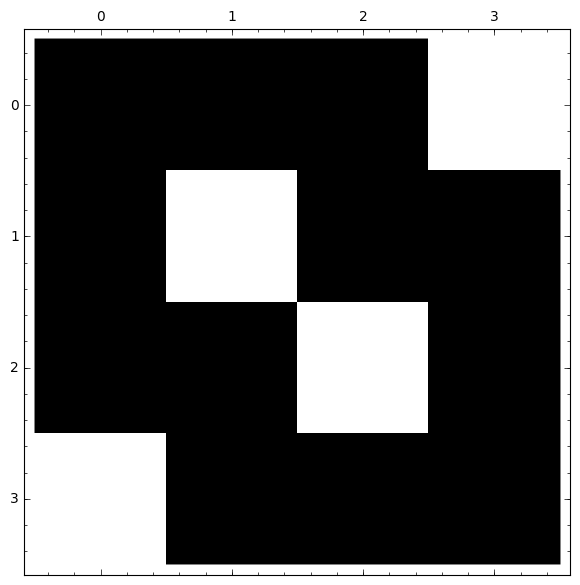
\includegraphics[width=.9\linewidth]{../matrix_plot/re2_1_weight_class_matrix.png}
  \captionof{figure}{$[f_{2,1}]$: weight classes}
  \label{fig:c2_1_weight_class_matrix}
\end{minipage}%
\begin{minipage}{.48\textwidth}
  \centering
  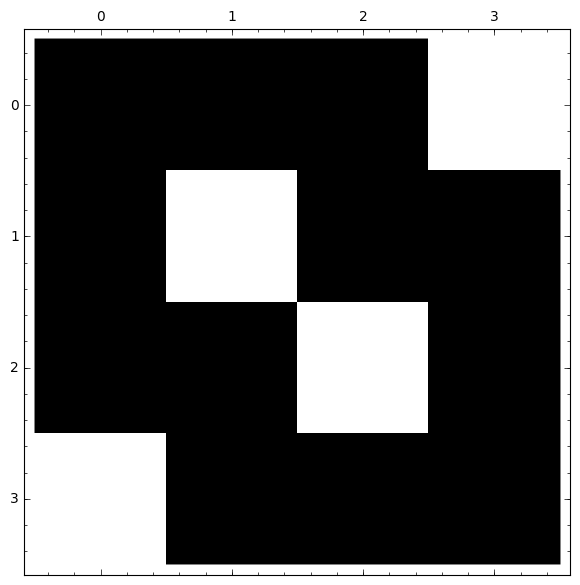
\includegraphics[width=.9\linewidth]{../matrix_plot/re2_1_bent_cayley_graph_index_matrix.png}
  \captionof{figure}{$[f_{2,1}]$: extended Cayley classes}
  \label{fig:c2_1_bent_cayley_graph_index_matrix}
\end{minipage}
\end{figure}

% \end{frame}
% \begin{frame}
\subsection{Bent functions in 4 dimensions}

The bent functions on $\Z_2^4$ consist of one extended affine class, containing the extended translation class $[f_{4,1}]$ where
$f_{4,1}(x) := x_0 x_1 + x_2 x_3$ is self dual.

~

Two extended Cayley classes:
\begin{align*}
\def\arraystretch{1.2}
\begin{array}{|cccl|}
\hline
\text{Class} &
\text{Parameters} &
\text{2-rank} &
\text{Clique polynomial}
\\
\hline
0 &
(16, 6, 2, 2) &
6 &
\begin{array}{l}
8t^{4} + 32t^{3} + 48t^{2} + 16t + 1
\end{array}
\\
1 &
(16, 10, 6, 6) &
6 &
\begin{array}{l}
16t^{5} + 120t^{4} + 160t^{3}
\,+
\\
 80t^{2} + 16t + 1
\end{array}
\\
\hline
\end{array}
\end{align*}

The Cayley graphs for classes 1 and 2 are isomorphic to those those obtained from the following
projective two-weight codes:

\begin{align*}
\begin{array}{|ccc|}
\hline
\text{Class} &
\text{Parameters} & \text{Generator matrix}
\\
\hline
1 &
[6, 4, 2] &
\left[
\begin{array}{cccccc}
0 & 0 & 1 & 1 & 1 & 1
\\
1 & 0 & 0 & 1 & 1 & 1
\\
1 & 1 & 1 & 1 & 0 & 0
\\
0 & 1 & 1 & 1 & 1 & 0
\end{array}
\right]
\\
2 &
[5, 4, 2] &
\left[
\begin{array}{ccccc}
1 & 1 & 0 & 0 & 0
\\
0 & 1 & 1 & 0 & 0
\\
0 & 0 & 0 & 1 & 1
\\
1 & 0 & 0 & 0 & 1
\end{array}
\right]
\\
\hline
\end{array}
\end{align*}

\begin{figure}[!hb]
\centering
\begin{minipage}{.48\textwidth}
  \centering
  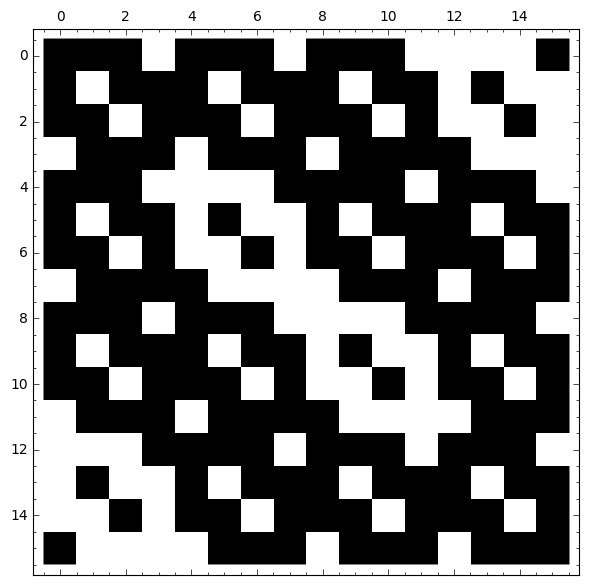
\includegraphics[width=.9\linewidth]{../matrix_plot/re4_1_weight_class_matrix.png}
  \captionof{figure}{$[f_{4,1}]$: weight classes}
  \label{fig:c4_1_weight_class_matrix}
\end{minipage}%
\begin{minipage}{.48\textwidth}
  \centering
  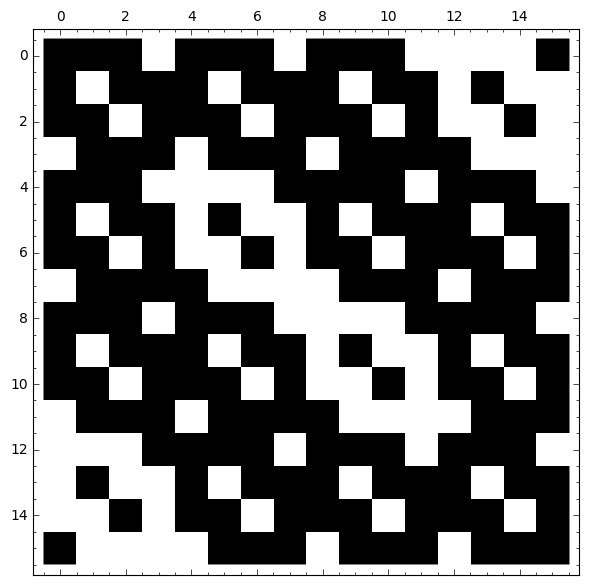
\includegraphics[width=.9\linewidth]{../matrix_plot/re4_1_bent_cayley_graph_index_matrix.png}
  \captionof{figure}{$[f_{4,1}]$: extended Cayley classes}
  \label{fig:c4_1_bent_cayley_graph_index_matrix}
\end{minipage}
\end{figure}

% \end{frame}
% \begin{frame}
\subsection{Bent functions in 6 dimensions}
\paragraph*{Extended affine classes.}

The bent functions on $\Z_2^4$ consist of four
extended affine classes, containing the following extended translation classes:

\begin{align*}
\def\arraystretch{1.2}
\begin{array}{|cl|}
\hline
\text{Class} &
\text{Representative}
\\
\hline
\,[f_{6,1}] & f_{6,1} :=
\begin{array}{l}
x_{0} x_{1} + x_{2} x_{3} + x_{4} x_{5}
\end{array}
\\
\,[f_{6,2}] & f_{6,2} :=
\begin{array}{l}
x_{0} x_{1} x_{2} + x_{0} x_{3} + x_{1} x_{4} + x_{2} x_{5}
\end{array}
\\
\,[f_{6,3}] & f_{6,3} :=
\begin{array}{l}
x_{0} x_{1} x_{2} + x_{0} x_{1} + x_{0} x_{3} + x_{1} x_{3} x_{4} + x_{1} x_{5} +
\\
x_{2} x_{4} + x_{3} x_{4}
\end{array}
\\
\,[f_{6,4}] & f_{6,4} :=
\begin{array}{l}
x_{0} x_{1} x_{2} + x_{0} x_{3} + x_{1} x_{3} x_{4} + x_{1} x_{5} + x_{2} x_{3} x_{5} +
\\
x_{2} x_{3} + x_{2} x_{4} + x_{2} x_{5} + x_{3} x_{4} + x_{3} x_{5}
\end{array}
\\
\hline
\end{array}
\end{align*}

In 1996, Tonchev classified the binary projective two-weight $[27,21,3]$ and $[35,6,16]$ codes
listing them in Tables 1 and 2, respectively, of his paper \cite{Ton96uniformly}.
These tables are repeated as Tables 1.155 and 1.156 in Chapter VII.1 of the Handbook of
Combinatorial Designs, Second Edition \cite{Ton07codes},
with a different numbering.
For each of the codes listed in these two tables, the characteristics of the corresponding
strongly regular graph is also listed.

In the classification given below, the Cayley graph of each Cayley class is matched by isomorphism
with a strongly regular graph corresponding to one
or more of Tonchev's projective two-weight codes, or the complement of such a graph.

% \end{frame}
% \begin{frame}
\paragraph*{ET class $[f_{6,1}]$.}

The function
$f_{6,1}(x) = x_0 x_1 + x_2 x_3 + x_4 x_5$ is self dual.

The extended translation class contains
two extended Cayley classes:

\small{}
\begin{align*}
\def\arraystretch{1.2}
\begin{array}{|cccl|}
\hline
\text{Class} &
\text{Parameters} &
\text{2-rank} &
\text{Clique polynomial}
\\
\hline
0 &
(64, 28, 12, 12) &
8 &
\begin{array}{l}
64t^{8} + 512t^{7} + 1792t^{6}
\,+
\\
 3584t^{5} + 5376t^{4} + 3584t^{3}
\,+
\\
 896t^{2} + 64t + 1
\end{array}
\\
1 &
(64, 36, 20, 20) &
8 &
\begin{array}{l}
2304t^{6} + 13824t^{5} + 19200t^{4}
\,+
\\
 7680t^{3} + 1152t^{2} + 64t + 1
\end{array}
\\
\hline
\end{array}
\end{align*}

The Cayley graphs for classes 0 and 1 are isomorphic to those those obtained from the following
projective two-weight
codes as listed by Tonchev \cite{Ton07codes}:

\begin{align*}
\def\arraystretch{1.2}
\begin{array}{|ccl|}
\hline
\text{Class} &
\text{Parameters} & \text{Reference}
\\
\hline
0 & [35,6,16] & \text{Table 1.156 1, 2 (complement)}
\\
1 & [27,6,12] & \text{Table 1.155 1 }
\\
\hline
\end{array}
\end{align*}

%\slidecite{Tonchev 1996, 2006}
% \end{frame}
% \begin{frame}
\paragraph*{ET class $[f_{6,2}]$.}

This is the extended translation class of the bent function
$f_{6,2}(x) = x_{0} x_{1} x_{2} + x_{0} x_{3} + x_{1} x_{4} + x_{2} x_{5}$.

The extended translation class contains
three extended Cayley classes:
\small{}
\begin{align*}
\def\arraystretch{1.2}
\begin{array}{|cccl|}
\hline
\text{Class} &
\text{Parameters} &
\text{2-rank} &
\text{Clique polynomial}
\\
\hline
0 &
(64, 28, 12, 12) &
8 &
\begin{array}{l}
64t^{8} + 512t^{7} + 1792t^{6}
\,+
\\
 3584t^{5} + 5376t^{4} + 3584t^{3}
\,+
\\
 896t^{2} + 64t + 1
\end{array}
\\
1 &
(64, 28, 12, 12) &
8 &
\begin{array}{l}
256t^{6} + 1536t^{5} + 4352t^{4}
\,+
\\
 3584t^{3} + 896t^{2} + 64t + 1
\end{array}
\\
2 &
(64, 36, 20, 20) &
8 &
\begin{array}{l}
192t^{8} + 1536t^{7} + 8960t^{6}
\,+
\\
 19968t^{5} + 20224t^{4} + 7680t^{3}
\,+
\\
 1152t^{2} + 64t + 1
\end{array}
\\
\hline
\end{array}
\end{align*}


Graph 0 is isomorphic to graph 0 of ET class $[f_{6,1}]$,
and is also isomorphic to the complement of Royle's $(64,35,18,20)$ strongly regular graph $X$
\cite{Roy08normal}.
%
%~
%
%\slidecite{Royle 2008}
% \end{frame}
% \begin{frame}
%\paragraph*{ET class $[f_{6,2}]$: two-weight codes.}

The Cayley graphs for classes 0 to 2 are isomorphic to those those obtained from the following
projective two-weight
codes as listed by Tonchev \cite{Ton07codes}:

\begin{align*}
\def\arraystretch{1.2}
\begin{array}{|ccl|}
\hline
\text{Class} &
\text{Parameters} & \text{Reference}
\\
\hline
0 & [35,6,16] & \text{Table 1.156 1, 2 (complement)}
\\
1 & [35,6,16] & \text{Table 1.156 3 (complement)}
\\
2 & [27,6,12] & \text{Table 1.155 2 }
\\
\hline
\end{array}
\end{align*}

%\slidecite{Tonchev 1996, 2006}
% \end{frame}
% \begin{frame}
\paragraph*{ET class $[f_{6,3}]$.}

This is the extended translation class of the bent function
\begin{align*}
f_{6,3}(x) &= x_{0} x_{1} x_{2} + x_{0} x_{1} + x_{0} x_{3} + x_{1} x_{3} x_{4}
\\
           &+ x_{1} x_{5} + x_{2} x_{4} + x_{3} x_{4}.
\end{align*}

The extended translation class contains
four extended Cayley classes:

\small{}
\begin{align*}
\def\arraystretch{1.2}
\begin{array}{|cccl|}
\hline
\text{Class} &
\text{Parameters} &
\text{2-rank} &
\text{Clique polynomial}
\\
\hline
0 &
(64, 28, 12, 12) &
12 &
\begin{array}{l}
32t^{8} + 256t^{7} + 896t^{6}
\,+
\\
 2048t^{5} + 4608t^{4} + 3584t^{3}
\,+
\\
 896t^{2} + 64t + 1
\end{array}
\\
1 &
(64, 36, 20, 20) &
12 &
\begin{array}{l}
160t^{8} + 1280t^{7} + 9344t^{6}
\,+
\\
 21504t^{5} + 20480t^{4} + 7680t^{3}
\,+
\\
 1152t^{2} + 64t + 1
\end{array}
\\
2 &
(64, 28, 12, 12) &
12 &
\begin{array}{l}
64t^{6} + 1024t^{5} + 4096t^{4}
\,+
\\
 3584t^{3} + 896t^{2} + 64t + 1
\end{array}
\\
3 &
(64, 36, 20, 20) &
12 &
\begin{array}{l}
160t^{8} + 1664t^{7} + 9792t^{6}
\,+
\\
 21504t^{5} + 20480t^{4} + 7680t^{3}
\,+
\\
 1152t^{2} + 64t + 1
\end{array}
\\
\hline
\end{array}
\end{align*}

The Cayley graphs for classes 0 to 3 are isomorphic to those those obtained from the following
projective two-weight
codes as listed by Tonchev \cite{Ton07codes}:

\begin{align*}
\def\arraystretch{1.2}
\begin{array}{|ccl|}
\hline
\text{Class} &
\text{Parameters} & \text{Reference}
\\
\hline
0 & [35,6,16] & \text{Table 1.156 4 (complement)}
\\
1 & [27,6,12] & \text{Table 1.155 3 }
\\
2 & [35,6,16] & \text{Table 1.156 5 (complement)}
\\
3 & [27,6,12] & \text{Table 1.155 4 }
\\
\hline
\end{array}
\end{align*}

%\slidecite{Tonchev 1996, 2006}
% \end{frame}
% \begin{frame}
\paragraph*{ET class $[f_{6,4}]$.}

This is the extended translation class of the bent function
\begin{align*}
f_{6,4}(x) &= x_{0} x_{1} x_{2} + x_{0} x_{3} + x_{1} x_{3} x_{4} + x_{1} x_{5} + x_{2} x_{3} x_{5}
\\
           &+ x_{2} x_{3} + x_{2} x_{4} + x_{2} x_{5} + x_{3} x_{4} + x_{3} x_{5}.
\end{align*}

The extended translation class contains
three extended Cayley classes:
\small{}

\begin{align*}
\def\arraystretch{1.2}
\begin{array}{|cccl|}
\hline
\text{Class} &
\text{Parameters} &
\text{2-rank} &
\text{Clique polynomial}
\\
\hline
0 &
(64, 28, 12, 12) &
14 &
\begin{array}{l}
32t^{8} + 256t^{7} + 896t^{6}
\,+
\\
 1792t^{5} + 4480t^{4} + 3584t^{3}
\,+
\\
 896t^{2} + 64t + 1
\end{array}
\\
1 &
(64, 28, 12, 12) &
14 &
\begin{array}{l}
16t^{8} + 128t^{7} + 448t^{6}
\,+
\\
 1280t^{5} + 4224t^{4} + 3584t^{3}
\,+
\\
 896t^{2} + 64t + 1
\end{array}
\\
2 &
(64, 36, 20, 20) &
14 &
\begin{array}{l}
176t^{8} + 1408t^{7} + 9664t^{6}
\,+
\\
 22272t^{5} + 20608t^{4} + 7680t^{3}
\,+
\\
 1152t^{2} + 64t + 1
\end{array}
\\
\hline
\end{array}
\end{align*}

The Cayley graphs for classes 0 to 2 are isomorphic to those those obtained from the following
projective two-weight
codes as listed by Tonchev \cite{Ton07codes}:

\begin{align*}
\def\arraystretch{1.2}
\begin{array}{|ccl|}
\hline
\text{Class} &
\text{Parameters} & \text{Reference}
\\
\hline
0 & [35,6,16] & \text{Table 1.156 7 (complement)}
\\
1 & [35,6,16] & \text{Table 1.156 6 (complement)}
\\
2 & [27,6,12] & \text{Table 1.155 5 }
\\
\hline
\end{array}
\end{align*}

%\slidecite{Tonchev 1996, 2006}
% \end{frame}
% \begin{frame}

\subsection{Bent functions in 8 dimensions}

There are
$99 270 589 265 934 370 305 785 861 242 880 \approx 2^{106}$ bent functions in dimension 8,
according to Langevin and Leander \cite{LanL11counting}.
%
%~
%
The number of EA classes has not yet been published, let alone a list of representatives.

\paragraph*{Extended affine classes up to degree 3.}

Up to degree 3:
Ten extended affine classes, containing the following extended translation classes:

\small{}
\begin{align*}
\def\arraystretch{1.2}
\begin{array}{|cl|}
\hline
\text{Class} &
\text{Representative}
\\
\hline
\,[f_{ 8 , 1 }] & f_{ 8 , 1 } :=
\begin{array}{l}
x_{0} x_{1} + x_{2} x_{3} + x_{4} x_{5} + x_{6} x_{7}
\end{array}
\\
\,[f_{ 8 , 2 }] & f_{ 8 , 2 } :=
\begin{array}{l}
x_{0} x_{1} x_{2} + x_{0} x_{3} + x_{1} x_{4} + x_{2} x_{5} + x_{6} x_{7}
\end{array}
\\
\,[f_{ 8 , 3 }] & f_{ 8 , 3 } :=
\begin{array}{l}
x_{0} x_{1} x_{2} + x_{0} x_{6} + x_{1} x_{3} x_{4} + x_{1} x_{5} + x_{2} x_{3} + x_{4} x_{7}
\end{array}
\\
\,[f_{ 8 , 4 }] & f_{ 8 , 4 } :=
\begin{array}{l}
x_{0} x_{1} x_{2} + x_{0} x_{2} + x_{0} x_{4} + x_{1} x_{3} x_{4} + x_{1} x_{5} + x_{2} x_{3} +
x_{6} x_{7}
\end{array}
\\
\,[f_{ 8 , 5 }] & f_{ 8 , 5 } :=
\begin{array}{l}
x_{0} x_{1} x_{2} + x_{0} x_{6} + x_{1} x_{3} x_{4} + x_{1} x_{4} + x_{1} x_{5} + x_{2} x_{3} x_{5}
+ x_{2} x_{4} + x_{3} x_{7}
\end{array}
\\
\,[f_{ 8 , 6 }] & f_{ 8 , 6 } :=
\begin{array}{l}
x_{0} x_{1} x_{2} + x_{0} x_{2} + x_{0} x_{3} + x_{1} x_{3} x_{4} + x_{1} x_{6} + x_{2} x_{3} x_{5}
+ x_{2} x_{4} + x_{5} x_{7}
\end{array}
\\
\,[f_{ 8 , 7 }] & f_{ 8 , 7 } :=
\begin{array}{l}
x_{0} x_{1} x_{2} + x_{0} x_{1} + x_{0} x_{2} + x_{0} x_{3} + x_{1} x_{3} x_{4} + x_{1} x_{4} +
x_{1} x_{5} + x_{2} x_{3} x_{5}
\\
+\,  x_{2} x_{4} + x_{6} x_{7}
\end{array}
\\
\,[f_{ 8 , 8 }] & f_{ 8 , 8 } :=
\begin{array}{l}
x_{0} x_{1} x_{2} + x_{0} x_{5} + x_{1} x_{3} x_{4} + x_{1} x_{6} + x_{2} x_{3} x_{5} + x_{2} x_{4}
+ x_{3} x_{7}
\end{array}
\\
\,[f_{ 8 , 9 }] & f_{ 8 , 9 } :=
\begin{array}{l}
x_{0} x_{1} x_{6} + x_{0} x_{3} + x_{1} x_{4} + x_{2} x_{3} x_{6} + x_{2} x_{5} + x_{3} x_{4} +
x_{4} x_{5} x_{6} + x_{6} x_{7}
\end{array}
\\
\,[f_{ 8 , 10 }] & f_{ 8 , 10 } :=
\begin{array}{l}
x_{0} x_{1} x_{2} + x_{0} x_{3} x_{6} + x_{0} x_{4} + x_{0} x_{5} + x_{1} x_{3} x_{4} + x_{1} x_{6}
+ x_{2} x_{3} x_{5}
\\
+\, x_{2} x_{4} + x_{3} x_{7}
\end{array}
\\
\hline
\end{array}
\end{align*}
\normalsize{}
% \end{frame}
% \begin{frame}
\paragraph*{ET class $[f_{8,1}]$.}

% f8_1
\small{}
\begin{align*}
\def\arraystretch{1.2}
\begin{array}{|cccl|}
\hline
\text{Class} &
\text{Parameters} &
\text{2-rank} &
\text{Clique polynomial}
\\
\hline
0 &
(256, 120, 56, 56) &
10 &
\begin{array}{l}
245760t^{9} + 3317760t^{8}
\,+
\\
 8847360t^{7} + 10321920t^{6}
\,+
\\
 6193152t^{5} + 2007040t^{4}
\,+
\\
 286720t^{3} + 15360t^{2} + 256t + 1
\end{array}
\\
1 &
(256, 136, 72, 72) &
10 &
\begin{array}{l}
417792t^{8} + 3342336t^{7}
\,+
\\
 11698176t^{6} + 11698176t^{5}
\,+
\\
 3760128t^{4} + 417792t^{3}
\,+
\\
 17408t^{2} + 256t + 1
\end{array}
\\
\hline
\end{array}
\end{align*}

\begin{figure}[!hb]
\centering
\begin{minipage}{.48\textwidth}
  \centering
  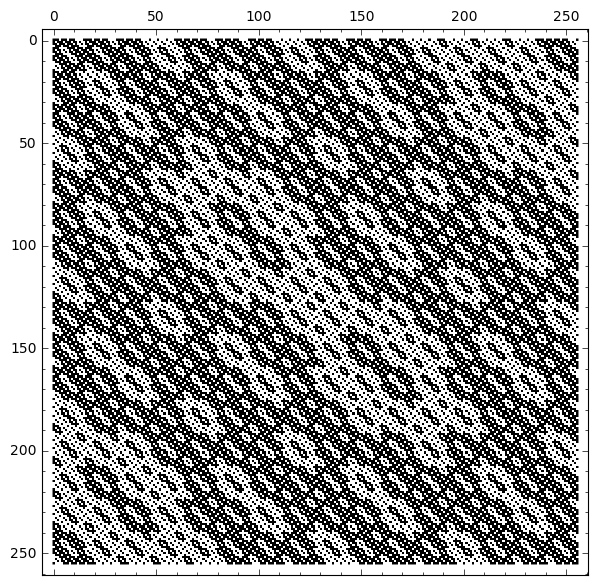
\includegraphics[width=.9\linewidth]{../matrix_plot/re8_1_weight_class_matrix.png}
  \captionof{figure}{$[f_{8,1}]$: weight classes}
  \label{fig:8_1_weight_class_matrix}
\end{minipage}%
\begin{minipage}{.48\textwidth}
  \centering
  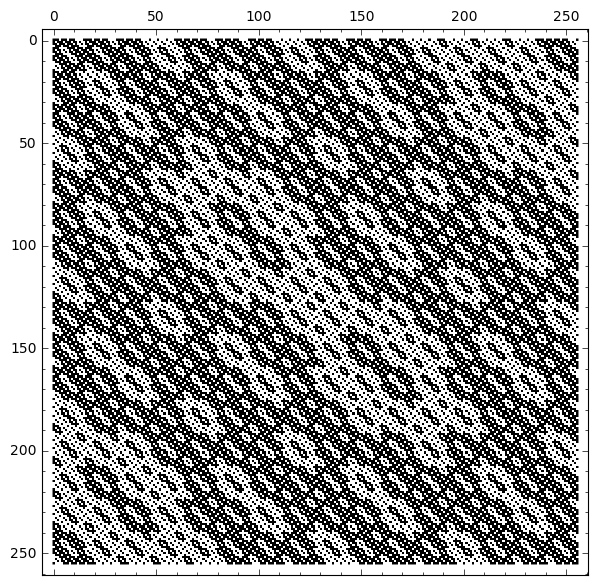
\includegraphics[width=.9\linewidth]{../matrix_plot/re8_1_bent_cayley_graph_index_matrix.png}
  \captionof{figure}{$[f_{8,1}]$: 2 extended Cayley classes}
  \label{fig:8_1_bent_cayley_graph_index_matrix}
\end{minipage}
\end{figure}
~
% \end{frame}
% \begin{frame}
\paragraph*{ET class $[f_{8,2}]$.}

% f8_2
\small{}
\begin{align*}
\def\arraystretch{1.2}
\begin{array}{|cccl|}
\hline
\text{Class} &
\text{Parameters} &
\text{2-rank} &
\text{Clique polynomial}
\\
\hline
0 &
(256, 120, 56, 56) &
10 &
\begin{array}{l}
245760t^{9} + 3317760t^{8}
\,+
\\
 8847360t^{7} + 10321920t^{6}
\,+
\\
 6193152t^{5} + 2007040t^{4}
\,+
\\
 286720t^{3} + 15360t^{2} + 256t + 1
\end{array}
\\
1 &
(256, 120, 56, 56) &
10 &
\begin{array}{l}
49152t^{9} + 663552t^{8}
\,+
\\
 2555904t^{7} + 5079040t^{6}
\,+
\\
 4620288t^{5} + 1875968t^{4}
\,+
\\
 286720t^{3} + 15360t^{2} + 256t + 1
\end{array}
\\
2 &
(256, 136, 72, 72) &
10 &
\begin{array}{l}
327680t^{9} + 4055040t^{8}
\,+
\\
 13828096t^{7} + 22183936t^{6}
\,+
\\
 14319616t^{5} + 3891200t^{4}
\,+
\\
 417792t^{3} + 17408t^{2} + 256t + 1
\end{array}
\\
3 &
(256, 136, 72, 72) &
10 &
\begin{array}{l}
417792t^{8} + 3342336t^{7}
\,+
\\
 11698176t^{6} + 11698176t^{5}
\,+
\\
 3760128t^{4} + 417792t^{3}
\,+
\\
 17408t^{2} + 256t + 1
\end{array}
\\
\hline
\end{array}
\end{align*}


\begin{figure}[!hb]
\centering
\begin{minipage}{.48\textwidth}
  \centering
  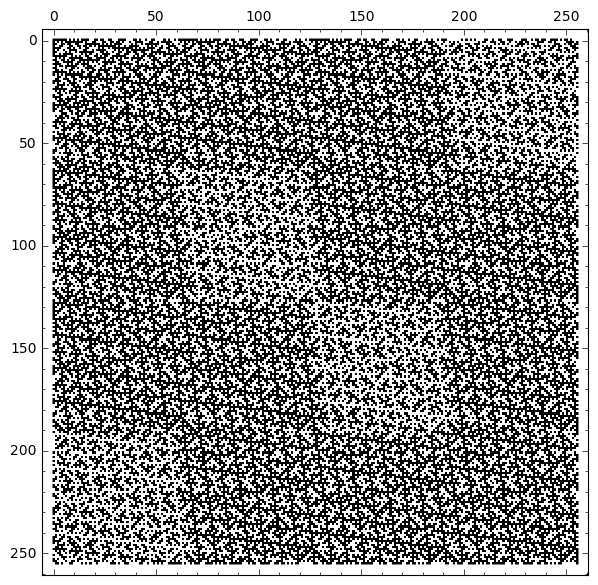
\includegraphics[width=.9\linewidth]{../matrix_plot/re8_2_weight_class_matrix.png}
  \captionof{figure}{$[f_{8,2}]$: weight classes}
  \label{fig:8_2_weight_class_matrix}
\end{minipage}%
\begin{minipage}{.48\textwidth}
  \centering
  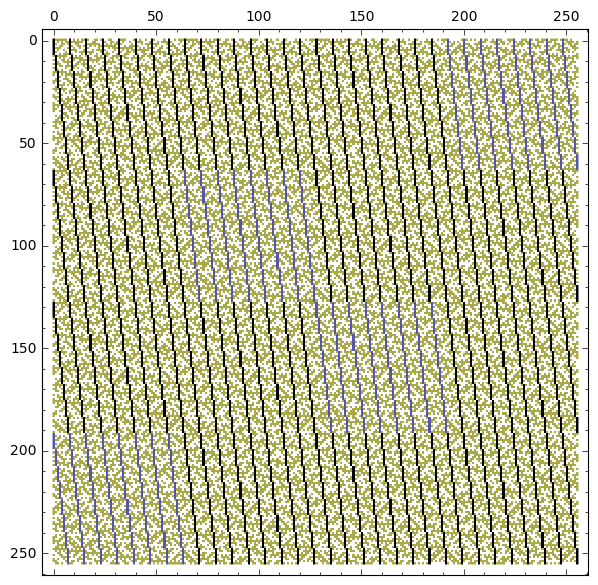
\includegraphics[width=.9\linewidth]{../matrix_plot/re8_2_bent_cayley_graph_index_matrix.png}
  \captionof{figure}{$[f_{8,2}]$: 4 extended Cayley classes}
  \label{fig:8_2_bent_cayley_graph_index_matrix}
\end{minipage}
\end{figure}
~
% \end{frame}
% \begin{frame}
\paragraph*{ET class $[f_{8,3}]$.}

% f8_3
\small{}
\begin{align*}
\def\arraystretch{1.2}
\begin{array}{|cccl|}
\hline
\text{Class} &
\text{Parameters} &
\text{2-rank} &
\text{Clique polynomial}
\\
\hline
0 &
(256, 120, 56, 56) &
12 &
\begin{array}{l}
81920t^{9} + 1368064t^{8}
\,+
\\
 4653056t^{7} + 7176192t^{6}
\,+
\\
 5406720t^{5} + 1941504t^{4}
\,+
\\
 286720t^{3} + 15360t^{2} + 256t + 1
\end{array}
\\
1 &
(256, 136, 72, 72) &
12 &
\begin{array}{l}
294912t^{9} + 6299648t^{8}
\,+
\\
 21692416t^{7} + 27951104t^{6}
\,+
\\
 15630336t^{5} + 3956736t^{4}
\,+
\\
 417792t^{3} + 17408t^{2} + 256t + 1
\end{array}
\\
2 &
(256, 120, 56, 56) &
12 &
\begin{array}{l}
16384t^{9} + 221184t^{8}
\,+
\\
 1277952t^{7} + 3768320t^{6}
\,+
\\
 4227072t^{5} + 1843200t^{4}
\,+
\\
 286720t^{3} + 15360t^{2} + 256t + 1
\end{array}
\\
3 &
(256, 136, 72, 72) &
12 &
\begin{array}{l}
262144t^{9} + 4399104t^{8}
\,+
\\
 16220160t^{7} + 24281088t^{6}
\,+
\\
 14974976t^{5} + 3923968t^{4}
\,+
\\
 417792t^{3} + 17408t^{2} + 256t + 1
\end{array}
\\
4 &
(256, 120, 56, 56) &
12 &
\begin{array}{l}
49152t^{9} + 729088t^{8}
\,+
\\
 2686976t^{7} + 5079040t^{6}
\,+
\\
 4620288t^{5} + 1875968t^{4}
\,+
\\
 286720t^{3} + 15360t^{2} + 256t + 1
\end{array}
\\
5 &
(256, 136, 72, 72) &
12 &
\begin{array}{l}
196608t^{9} + 3399680t^{8}
\,+
\\
 13172736t^{7} + 21659648t^{6}
\,+
\\
 14319616t^{5} + 3891200t^{4}
\,+
\\
 417792t^{3} + 17408t^{2} + 256t + 1
\end{array}
\\
\hline
\end{array}
\end{align*}

\begin{figure}[!hb]
\centering
\begin{minipage}{.48\textwidth}
  \centering
  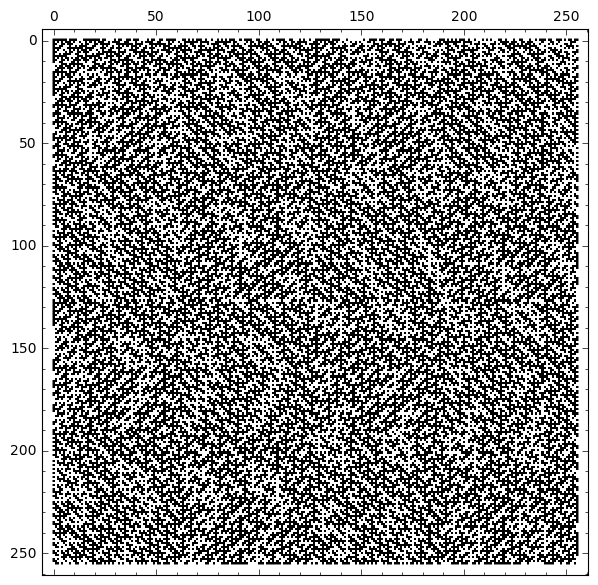
\includegraphics[width=.9\linewidth]{../matrix_plot/re8_3_weight_class_matrix.png}
  \captionof{figure}{$[f_{8,3}]$: weight classes}
  \label{fig:8_3_weight_class_matrix}
\end{minipage}%
\begin{minipage}{.48\textwidth}
  \centering
  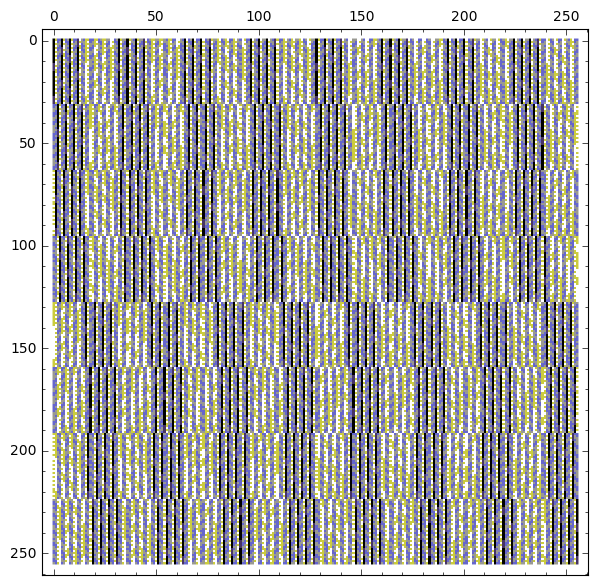
\includegraphics[width=.9\linewidth]{../matrix_plot/re8_3_bent_cayley_graph_index_matrix.png}
  \captionof{figure}{$[f_{8,3}]$: 6 extended Cayley classes}
  \label{fig:8_3_bent_cayley_graph_index_matrix}
\end{minipage}
\end{figure}
~
% \end{frame}
% \begin{frame}
\paragraph*{ET class $[f_{8,4}]$.}
% f8_4
\small{}
\begin{align*}
\def\arraystretch{1.2}
\begin{array}{|cccl|}
\hline
\text{Class} &
\text{Parameters} &
\text{2-rank} &
\text{Clique polynomial}
\\
\hline
0 &
(256, 120, 56, 56) &
14 &
\begin{array}{l}
69632t^{9} + 1099776t^{8}
\,+
\\
 3784704t^{7} + 6160384t^{6}
\,+
\\
 5013504t^{5} + 1908736t^{4}
\,+
\\
 286720t^{3} + 15360t^{2} + 256t + 1
\end{array}
\\
1 &
(256, 136, 72, 72) &
14 &
\begin{array}{l}
225280t^{9} + 4319232t^{8}
\,+
\\
 16203776t^{7} + 24313856t^{6}
\,+
\\
 14974976t^{5} + 3923968t^{4}
\,+
\\
 417792t^{3} + 17408t^{2} + 256t + 1
\end{array}
\\
2 &
(256, 120, 56, 56) &
14 &
\begin{array}{l}
1536t^{10} + 15360t^{9} + 209920t^{8}
\,+
\\
 1280000t^{7} + 3751936t^{6}
\,+
\\
 4227072t^{5} + 1843200t^{4}
\,+
\\
 286720t^{3} + 15360t^{2} + 256t + 1
\end{array}
\\
3 &
(256, 136, 72, 72) &
14 &
\begin{array}{l}
7680t^{10} + 230400t^{9}
\,+
\\
 4228096t^{8} + 16058368t^{7}
\,+
\\
 24166400t^{6} + 14974976t^{5}
\,+
\\
 3923968t^{4} + 417792t^{3}
\,+
\\
 17408t^{2} + 256t + 1
\end{array}
\\
4 &
(256, 136, 72, 72) &
14 &
\begin{array}{l}
110592t^{9} + 2344960t^{8}
\,+
\\
 10305536t^{7} + 18939904t^{6}
\,+
\\
 13664256t^{5} + 3858432t^{4}
\,+
\\
 417792t^{3} + 17408t^{2} + 256t + 1
\end{array}
\\
5 &
(256, 120, 56, 56) &
14 &
\begin{array}{l}
20480t^{9} + 337920t^{8}
\,+
\\
 1556480t^{7} + 3932160t^{6}
\,+
\\
 4227072t^{5} + 1843200t^{4}
\,+
\\
 286720t^{3} + 15360t^{2} + 256t + 1
\end{array}
\\
\hline
\end{array}
\end{align*}

\begin{figure}[!hb]
\centering
\begin{minipage}{.48\textwidth}
  \centering
  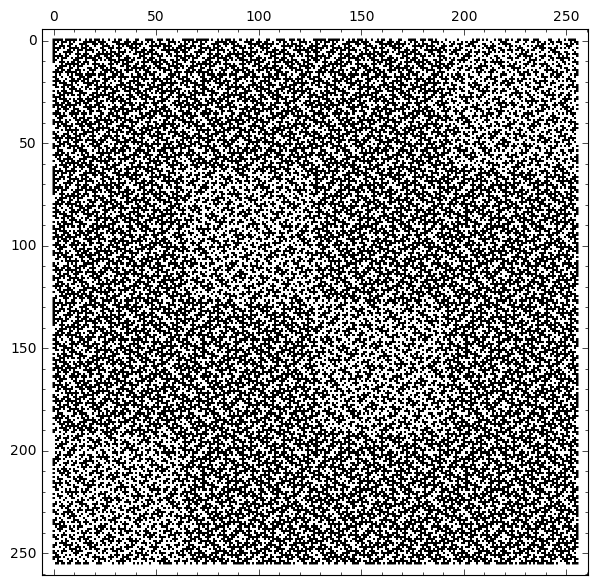
\includegraphics[width=.9\linewidth]{../matrix_plot/re8_4_weight_class_matrix.png}
  \captionof{figure}{$[f_{8,4}]$: weight classes}
  \label{fig:8_4_weight_class_matrix}
\end{minipage}%
\begin{minipage}{.48\textwidth}
  \centering
  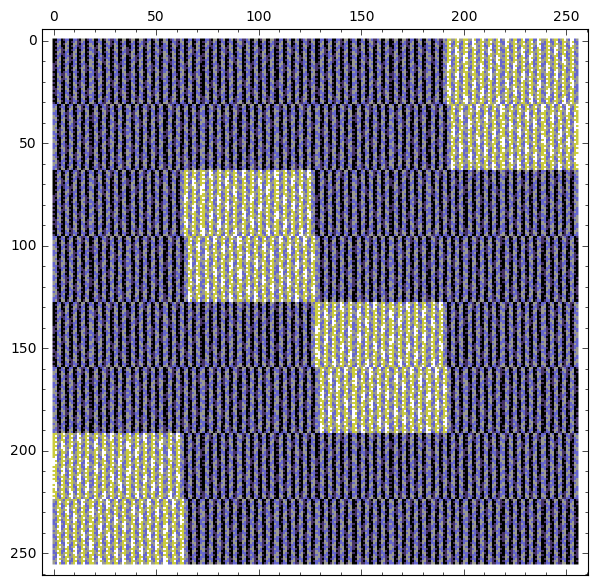
\includegraphics[width=.9\linewidth]{../matrix_plot/re8_4_bent_cayley_graph_index_matrix.png}
  \captionof{figure}{$[f_{8,4}]$: 5 extended Cayley classes}
  \label{fig:8_4_bent_cayley_graph_index_matrix}
\end{minipage}
\end{figure}
~
% \end{frame}
% \begin{frame}
\paragraph*{ET class $[f_{8,5}]$.}

% f8_5
\small{}
\begin{align*}
\def\arraystretch{1.2}
\begin{array}{|cccl|}
\hline
\text{Class} &
\text{Parameters} &
\text{2-rank} &
\text{Clique polynomial}
\\
\hline
0 &
(256, 120, 56, 56) &
14 &
\begin{array}{l}
32768t^{9} + 731136t^{8}
\,+
\\
 3096576t^{7} + 5767168t^{6}
\,+
\\
 5013504t^{5} + 1908736t^{4}
\,+
\\
 286720t^{3} + 15360t^{2} + 256t + 1
\end{array}
\\
1 &
(256, 120, 56, 56) &
14 &
\begin{array}{l}
28672t^{9} + 534528t^{8}
\,+
\\
 2211840t^{7} + 4718592t^{6}
\,+
\\
 4620288t^{5} + 1875968t^{4}
\,+
\\
 286720t^{3} + 15360t^{2} + 256t + 1
\end{array}
\\
2 &
(256, 136, 72, 72) &
14 &
\begin{array}{l}
159744t^{9} + 4753408t^{8}
\,+
\\
 19021824t^{7} + 26804224t^{6}
\,+
\\
 15630336t^{5} + 3956736t^{4}
\,+
\\
 417792t^{3} + 17408t^{2} + 256t + 1
\end{array}
\\
3 &
(256, 120, 56, 56) &
14 &
\begin{array}{l}
24576t^{9} + 526336t^{8}
\,+
\\
 2342912t^{7} + 4849664t^{6}
\,+
\\
 4620288t^{5} + 1875968t^{4}
\,+
\\
 286720t^{3} + 15360t^{2} + 256t + 1
\end{array}
\\
4 &
(256, 136, 72, 72) &
14 &
\begin{array}{l}
90112t^{9} + 2795520t^{8}
\,+
\\
 12402688t^{7} + 21168128t^{6}
\,+
\\
 14319616t^{5} + 3891200t^{4}
\,+
\\
 417792t^{3} + 17408t^{2} + 256t + 1
\end{array}
\\
5 &
(256, 120, 56, 56) &
14 &
\begin{array}{l}
16384t^{9} + 284672t^{8}
\,+
\\
 1392640t^{7} + 3735552t^{6}
\,+
\\
 4227072t^{5} + 1843200t^{4}
\,+
\\
 286720t^{3} + 15360t^{2} + 256t + 1
\end{array}
\\
\hline
\end{array}
\end{align*}
\newpage
\small{}
\begin{align*}
\def\arraystretch{1.2}
\begin{array}{|cccl|}
\hline
\text{Class} &
\text{Parameters} &
\text{2-rank} &
\text{Clique polynomial}
\\
\hline
6 &
(256, 136, 72, 72) &
14 &
\begin{array}{l}
131072t^{9} + 3577856t^{8}
\,+
\\
 15319040t^{7} + 23855104t^{6}
\,+
\\
 14974976t^{5} + 3923968t^{4}
\,+
\\
 417792t^{3} + 17408t^{2} + 256t + 1
\end{array}
\\
7 &
(256, 120, 56, 56) &
14 &
\begin{array}{l}
1536t^{10} + 19456t^{9} + 279552t^{8}
\,+
\\
 1394688t^{7} + 3751936t^{6}
\,+
\\
 4227072t^{5} + 1843200t^{4}
\,+
\\
 286720t^{3} + 15360t^{2} + 256t + 1
\end{array}
\\
8 &
(256, 136, 72, 72) &
14 &
\begin{array}{l}
5632t^{10} + 148480t^{9}
\,+
\\
 3621888t^{8} + 15206400t^{7}
\,+
\\
 23773184t^{6} + 14974976t^{5}
\,+
\\
 3923968t^{4} + 417792t^{3}
\,+
\\
 17408t^{2} + 256t + 1
\end{array}
\\
\hline
\end{array}
\end{align*}

\begin{figure}[!hb]
\centering
\begin{minipage}{.48\textwidth}
  \centering
  \includegraphics[width=.9\linewidth]{../matrix_plot/re8_5_weight_class_matrix.png}
  \captionof{figure}{$[f_{8,5}]$: weight classes}
  \label{fig:8_5_weight_class_matrix}
\end{minipage}%
\begin{minipage}{.48\textwidth}
  \centering
  \includegraphics[width=.9\linewidth]{../matrix_plot/re8_5_bent_cayley_graph_index_matrix.png}
  \captionof{figure}{$[f_{8,5}]$: 9 extended Cayley classes}
  \label{fig:8_5_bent_cayley_graph_index_matrix}
\end{minipage}
\end{figure}
~
% \end{frame}
% \begin{frame}
\paragraph*{ET class $[f_{8,6}]$.}


% f8_6
\small{}
\begin{align*}
\def\arraystretch{1.2}
\begin{array}{|cccl|}
\hline
\text{Class} &
\text{Parameters} &
\text{2-rank} &
\text{Clique polynomial}
\\
\hline
0 &
(256, 120, 56, 56) &
14 &
\begin{array}{l}
32768t^{9} + 731136t^{8}
\,+
\\
 3096576t^{7} + 5767168t^{6}
\,+
\\
 5013504t^{5} + 1908736t^{4}
\,+
\\
 286720t^{3} + 15360t^{2} + 256t + 1
\end{array}
\\
1 &
(256, 120, 56, 56) &
14 &
\begin{array}{l}
28672t^{9} + 534528t^{8}
\,+
\\
 2211840t^{7} + 4718592t^{6}
\,+
\\
 4620288t^{5} + 1875968t^{4}
\,+
\\
 286720t^{3} + 15360t^{2} + 256t + 1
\end{array}
\\
2 &
(256, 136, 72, 72) &
14 &
\begin{array}{l}
159744t^{9} + 4753408t^{8}
\,+
\\
 19021824t^{7} + 26804224t^{6}
\,+
\\
 15630336t^{5} + 3956736t^{4}
\,+
\\
 417792t^{3} + 17408t^{2} + 256t + 1
\end{array}
\\
3 &
(256, 120, 56, 56) &
14 &
\begin{array}{l}
1536t^{10} + 19456t^{9} + 279552t^{8}
\,+
\\
 1394688t^{7} + 3751936t^{6}
\,+
\\
 4227072t^{5} + 1843200t^{4}
\,+
\\
 286720t^{3} + 15360t^{2} + 256t + 1
\end{array}
\\
4 &
(256, 136, 72, 72) &
14 &
\begin{array}{l}
5632t^{10} + 148480t^{9}
\,+
\\
 3621888t^{8} + 15206400t^{7}
\,+
\\
 23773184t^{6} + 14974976t^{5}
\,+
\\
 3923968t^{4} + 417792t^{3}
\,+
\\
 17408t^{2} + 256t + 1
\end{array}
\\
5 &
(256, 120, 56, 56) &
14 &
\begin{array}{l}
24576t^{9} + 526336t^{8}
\,+
\\
 2342912t^{7} + 4849664t^{6}
\,+
\\
 4620288t^{5} + 1875968t^{4}
\,+
\\
 286720t^{3} + 15360t^{2} + 256t + 1
\end{array}
\\
\hline
\end{array}
\end{align*}
\newpage
\small{}
\begin{align*}
\def\arraystretch{1.2}
\begin{array}{|cccl|}
\hline
\text{Class} &
\text{Parameters} &
\text{2-rank} &
\text{Clique polynomial}
\\
\hline
6 &
(256, 120, 56, 56) &
14 &
\begin{array}{l}
16384t^{9} + 284672t^{8}
\,+
\\
 1392640t^{7} + 3735552t^{6}
\,+
\\
 4227072t^{5} + 1843200t^{4}
\,+
\\
 286720t^{3} + 15360t^{2} + 256t + 1
\end{array}
\\
7 &
(256, 136, 72, 72) &
14 &
\begin{array}{l}
131072t^{9} + 3577856t^{8}
\,+
\\
 15319040t^{7} + 23855104t^{6}
\,+
\\
 14974976t^{5} + 3923968t^{4}
\,+
\\
 417792t^{3} + 17408t^{2} + 256t + 1
\end{array}
\\
8 &
(256, 136, 72, 72) &
14 &
\begin{array}{l}
90112t^{9} + 2795520t^{8}
\,+
\\
 12402688t^{7} + 21168128t^{6}
\,+
\\
 14319616t^{5} + 3891200t^{4}
\,+
\\
 417792t^{3} + 17408t^{2} + 256t + 1
\end{array}
\\
\hline
\end{array}
\end{align*}

\begin{figure}[!hb]
\centering
\begin{minipage}{.48\textwidth}
  \centering
  \includegraphics[width=.9\linewidth]{../matrix_plot/re8_6_weight_class_matrix.png}
  \captionof{figure}{$[f_{8,6}]$: weight classes}
  \label{fig:8_6_weight_class_matrix}
\end{minipage}%
\begin{minipage}{.48\textwidth}
  \centering
  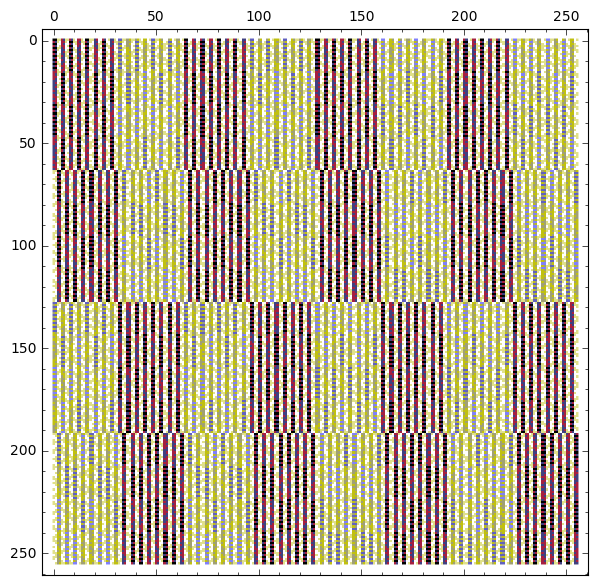
\includegraphics[width=.9\linewidth]{../matrix_plot/re8_6_bent_cayley_graph_index_matrix.png}
  \captionof{figure}{$[f_{8,6}]$: 9 extended Cayley classes}
  \label{fig:8_6_bent_cayley_graph_index_matrix}
\end{minipage}
\end{figure}
The same 9 classes as $[f_{8,5}]$, with the same frequencies!
% \end{frame}
% \begin{frame}
\paragraph*{ET class $[f_{8,7}]$.}
% f8_7
\small{}
\begin{align*}
\def\arraystretch{1.2}
\begin{array}{|cccl|}
\hline
\text{Class} &
\text{Parameters} &
\text{2-rank} &
\text{Clique polynomial}
\\
\hline
0 &
(256, 120, 56, 56) &
16 &
\begin{array}{l}
29696t^{9} + 655360t^{8}
\,+
\\
 2789376t^{7} + 5332992t^{6}
\,+
\\
 4816896t^{5} + 1892352t^{4}
\,+
\\
 286720t^{3} + 15360t^{2} + 256t + 1
\end{array}
\\
1 &
(256, 120, 56, 56) &
16 &
\begin{array}{l}
20480t^{9} + 409600t^{8}
\,+
\\
 1837056t^{7} + 4235264t^{6}
\,+
\\
 4423680t^{5} + 1859584t^{4}
\,+
\\
 286720t^{3} + 15360t^{2} + 256t + 1
\end{array}
\\
2 &
(256, 136, 72, 72) &
16 &
\begin{array}{l}
143360t^{9} + 3981312t^{8}
\,+
\\
 16697344t^{7} + 25108480t^{6}
\,+
\\
 15302656t^{5} + 3940352t^{4}
\,+
\\
 417792t^{3} + 17408t^{2} + 256t + 1
\end{array}
\\
3 &
(256, 136, 72, 72) &
16 &
\begin{array}{l}
64512t^{9} + 2316288t^{8}
\,+
\\
 10932224t^{7} + 19783680t^{6}
\,+
\\
 13991936t^{5} + 3874816t^{4}
\,+
\\
 417792t^{3} + 17408t^{2} + 256t + 1
\end{array}
\\
4 &
(256, 136, 72, 72) &
16 &
\begin{array}{l}
92160t^{9} + 2979840t^{8}
\,+
\\
 13608960t^{7} + 22388736t^{6}
\,+
\\
 14647296t^{5} + 3907584t^{4}
\,+
\\
 417792t^{3} + 17408t^{2} + 256t + 1
\end{array}
\\
5 &
(256, 120, 56, 56) &
16 &
\begin{array}{l}
6144t^{9} + 124928t^{8} + 944128t^{7}
\,+
\\
 3219456t^{6} + 4030464t^{5}
\,+
\\
 1826816t^{4} + 286720t^{3}
\,+
\\
 15360t^{2} + 256t + 1
\end{array}
\\
\hline
\end{array}
\end{align*}

\begin{figure}[!hb]
\centering
\begin{minipage}{.48\textwidth}
  \centering
  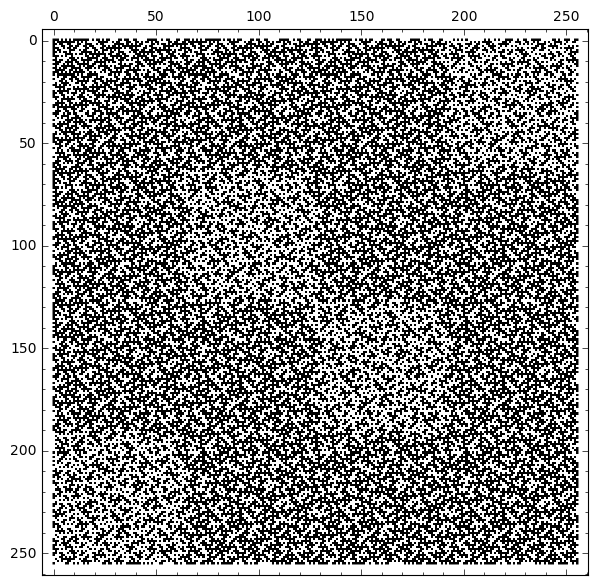
\includegraphics[width=.9\linewidth]{../matrix_plot/re8_7_weight_class_matrix.png}
  \captionof{figure}{$[f_{8,7}]$: weight classes}
  \label{fig:8_7_weight_class_matrix}
\end{minipage}%
\begin{minipage}{.48\textwidth}
  \centering
  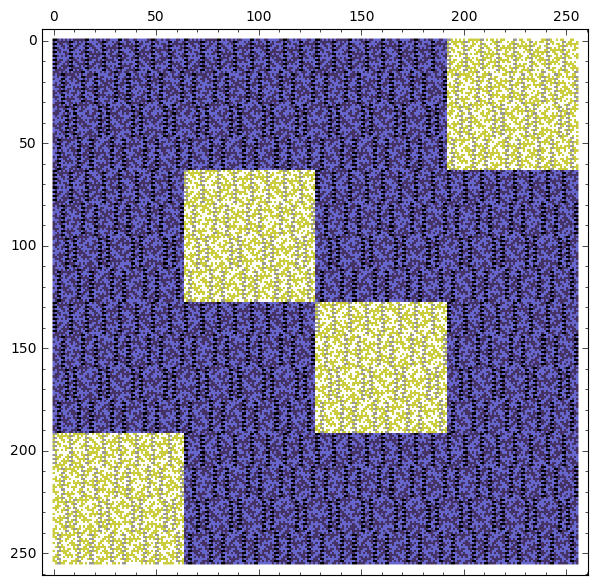
\includegraphics[width=.9\linewidth]{../matrix_plot/re8_7_bent_cayley_graph_index_matrix.png}
  \captionof{figure}{$[f_{8,7}]$: 5 extended Cayley classes}
  \label{fig:8_7_bent_cayley_graph_index_matrix}
\end{minipage}
\end{figure}
~
% \end{frame}
% \begin{frame}
\paragraph*{ET class $[f_{8,8}]$.}
% f8_8
\small{}
\begin{align*}
\def\arraystretch{1.2}
\begin{array}{|cccl|}
\hline
\text{Class} &
\text{Parameters} &
\text{2-rank} &
\text{Clique polynomial}
\\
\hline
0 &
(256, 120, 56, 56) &
14 &
\begin{array}{l}
32768t^{9} + 712704t^{8}
\,+
\\
 3014656t^{7} + 5734400t^{6}
\,+
\\
 5013504t^{5} + 1908736t^{4}
\,+
\\
 286720t^{3} + 15360t^{2} + 256t + 1
\end{array}
\\
1 &
(256, 120, 56, 56) &
14 &
\begin{array}{l}
24576t^{9} + 466944t^{8}
\,+
\\
 2064384t^{7} + 4685824t^{6}
\,+
\\
 4620288t^{5} + 1875968t^{4}
\,+
\\
 286720t^{3} + 15360t^{2} + 256t + 1
\end{array}
\\
2 &
(256, 136, 72, 72) &
14 &
\begin{array}{l}
172032t^{9} + 5332992t^{8}
\,+
\\
 20283392t^{7} + 27295744t^{6}
\,+
\\
 15630336t^{5} + 3956736t^{4}
\,+
\\
 417792t^{3} + 17408t^{2} + 256t + 1
\end{array}
\\
3 &
(256, 136, 72, 72) &
14 &
\begin{array}{l}
147456t^{9} + 3858432t^{8}
\,+
\\
 15990784t^{7} + 24150016t^{6}
\,+
\\
 14974976t^{5} + 3923968t^{4}
\,+
\\
 417792t^{3} + 17408t^{2} + 256t + 1
\end{array}
\\
4 &
(256, 120, 56, 56) &
14 &
\begin{array}{l}
16384t^{9} + 270336t^{8}
\,+
\\
 1376256t^{7} + 3768320t^{6}
\,+
\\
 4227072t^{5} + 1843200t^{4}
\,+
\\
 286720t^{3} + 15360t^{2} + 256t + 1
\end{array}
\\
5 &
(256, 136, 72, 72) &
14 &
\begin{array}{l}
163840t^{9} + 3858432t^{8}
\,+
\\
 15532032t^{7} + 23887872t^{6}
\,+
\\
 14974976t^{5} + 3923968t^{4}
\,+
\\
 417792t^{3} + 17408t^{2} + 256t + 1
\end{array}
\\
\hline
\end{array}
\end{align*}


\begin{figure}[!hb]
\centering
\begin{minipage}{.48\textwidth}
  \centering
  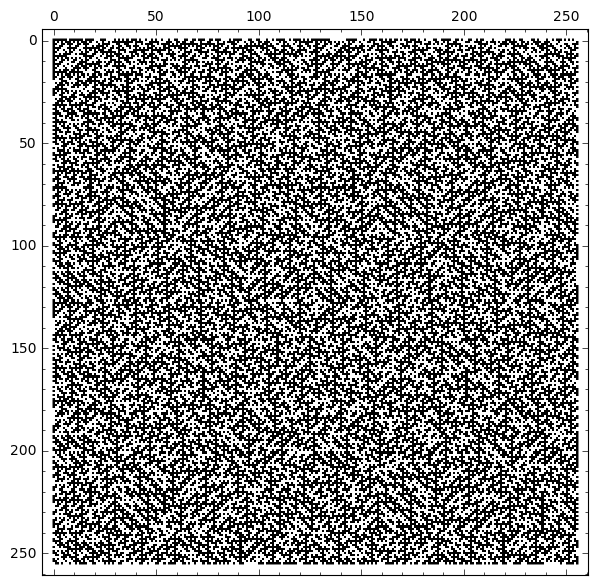
\includegraphics[width=.9\linewidth]{../matrix_plot/re8_8_weight_class_matrix.png}
  \captionof{figure}{$[f_{8,8}]$: weight classes}
  \label{fig:8_8_weight_class_matrix}
\end{minipage}%
\begin{minipage}{.48\textwidth}
  \centering
  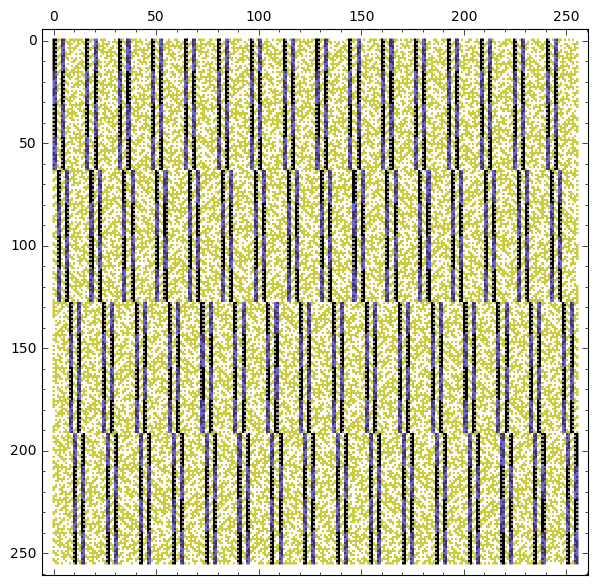
\includegraphics[width=.9\linewidth]{../matrix_plot/re8_8_bent_cayley_graph_index_matrix.png}
  \captionof{figure}{$[f_{8,8}]$: 6 extended Cayley classes}
  \label{fig:8_8_bent_cayley_graph_index_matrix}
\end{minipage}
\end{figure}
~
% \end{frame}
% \begin{frame}
\paragraph*{ET class $[f_{8,9}]$.}
% f8_9
\small{}
\begin{align*}
\def\arraystretch{1.2}
\begin{array}{|cccl|}
\hline
\text{Class} &
\text{Parameters} &
\text{2-rank} &
\text{Clique polynomial}
\\
\hline
0 &
(256, 120, 56, 56) &
16 &
\begin{array}{l}
45056t^{9} + 780288t^{8}
\,+
\\
 2998272t^{7} + 5505024t^{6}
\,+
\\
 4816896t^{5} + 1892352t^{4}
\,+
\\
 286720t^{3} + 15360t^{2} + 256t + 1
\end{array}
\\
1 &
(256, 120, 56, 56) &
16 &
\begin{array}{l}
45056t^{9} + 780288t^{8}
\,+
\\
 2998272t^{7} + 5505024t^{6}
\,+
\\
 4816896t^{5} + 1892352t^{4}
\,+
\\
 286720t^{3} + 15360t^{2} + 256t + 1
\end{array}
\\
2 &
(256, 136, 72, 72) &
16 &
\begin{array}{l}
184320t^{9} + 3852288t^{8}
\,+
\\
 14893056t^{7} + 23003136t^{6}
\,+
\\
 14647296t^{5} + 3907584t^{4}
\,+
\\
 417792t^{3} + 17408t^{2} + 256t + 1
\end{array}
\\
3 &
(256, 136, 72, 72) &
16 &
\begin{array}{l}
184320t^{9} + 3852288t^{8}
\,+
\\
 14893056t^{7} + 23003136t^{6}
\,+
\\
 14647296t^{5} + 3907584t^{4}
\,+
\\
 417792t^{3} + 17408t^{2} + 256t + 1
\end{array}
\\
4 &
(256, 120, 56, 56) &
16 &
\begin{array}{l}
105984t^{8} + 976896t^{7}
\,+
\\
 3440640t^{6} + 4128768t^{5}
\,+
\\
 1835008t^{4} + 286720t^{3}
\,+
\\
 15360t^{2} + 256t + 1
\end{array}
\\
5 &
(256, 136, 72, 72) &
16 &
\begin{array}{l}
9216t^{10} + 264192t^{9}
\,+
\\
 4468224t^{8} + 16803840t^{7}
\,+
\\
 24772608t^{6} + 15138816t^{5}
\,+
\\
 3932160t^{4} + 417792t^{3}
\,+
\\
 17408t^{2} + 256t + 1
\end{array}
\\
\hline
\end{array}
\end{align*}
\newpage
\small{}
\begin{align*}
\def\arraystretch{1.2}
\begin{array}{|cccl|}
\hline
\text{Class} &
\text{Parameters} &
\text{2-rank} &
\text{Clique polynomial}
\\
\hline
6 &
(256, 120, 56, 56) &
16 &
\begin{array}{l}
9216t^{9} + 124416t^{8} + 976896t^{7}
\,+
\\
 3440640t^{6} + 4128768t^{5}
\,+
\\
 1835008t^{4} + 286720t^{3}
\,+
\\
 15360t^{2} + 256t + 1
\end{array}
\\
7 &
(256, 136, 72, 72) &
16 &
\begin{array}{l}
193536t^{9} + 4449792t^{8}
\,+
\\
 16803840t^{7} + 24772608t^{6}
\,+
\\
 15138816t^{5} + 3932160t^{4}
\,+
\\
 417792t^{3} + 17408t^{2} + 256t + 1
\end{array}
\\
\hline
\end{array}
\end{align*}


\begin{figure}[!hb]
\centering
\begin{minipage}{.48\textwidth}
  \centering
  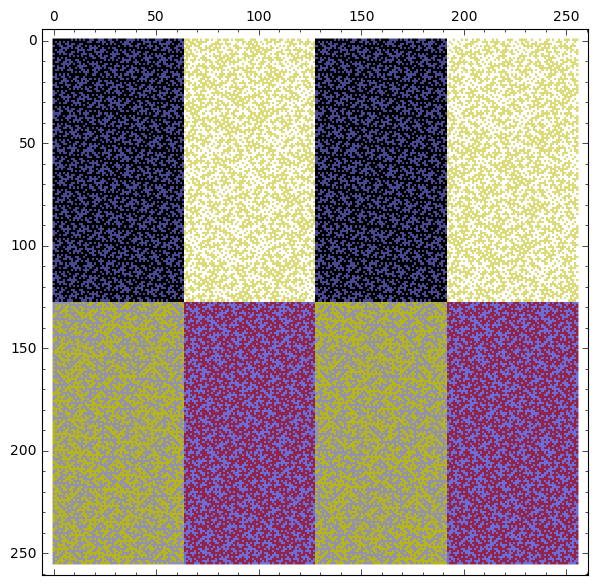
\includegraphics[width=.9\linewidth]{../matrix_plot/re8_9_bent_cayley_graph_index_matrix.png}
  \captionof{figure}{$[f_{8,9}]$: 8 extended Cayley classes ~~ ~~~~ ~~~~ ~~~~~~~~~}
  \label{fig:c8_9_bent_cayley_graph_index_matrix}
\end{minipage}
\begin{minipage}{.48\textwidth}
  \centering
  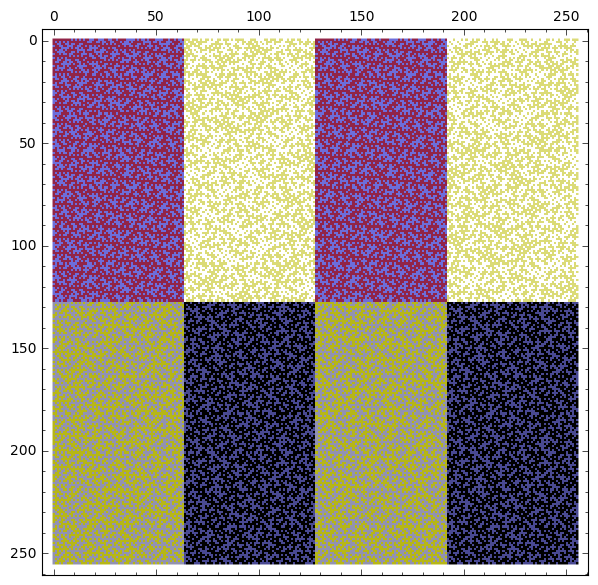
\includegraphics[width=.9\linewidth]{../matrix_plot/re8_9_dual_cayley_graph_index_matrix.png}
  \captionof{figure}{$[f_{8,9}]$: 8 extended Cayley classes of dual bent functions}
  \label{fig:c8_9_dual_cayley_graph_index_matrix}
\end{minipage}%
\end{figure}
4 of the 8 classes form 2 dual pairs of classes.
% \end{frame}
% \begin{frame}
\paragraph*{ET class $[f_{8,10}]$.}

% f8_10
\small{}
\begin{align*}
\def\arraystretch{1.2}
\begin{array}{|cccl|}
\hline
\text{Class} &
\text{Parameters} &
\text{2-rank} &
\text{Clique polynomial}
\\
\hline
0 &
(256, 120, 56, 56) &
16 &
\begin{array}{l}
16384t^{9} + 464896t^{8}
\,+
\\
 2310144t^{7} + 5046272t^{6}
\,+
\\
 4816896t^{5} + 1892352t^{4}
\,+
\\
 286720t^{3} + 15360t^{2} + 256t + 1
\end{array}
\\
1 &
(256, 120, 56, 56) &
16 &
\begin{array}{l}
16384t^{9} + 464896t^{8}
\,+
\\
 2310144t^{7} + 5046272t^{6}
\,+
\\
 4816896t^{5} + 1892352t^{4}
\,+
\\
 286720t^{3} + 15360t^{2} + 256t + 1
\end{array}
\\
2 &
(256, 120, 56, 56) &
16 &
\begin{array}{l}
12288t^{9} + 301056t^{8}
\,+
\\
 1589248t^{7} + 4128768t^{6}
\,+
\\
 4423680t^{5} + 1859584t^{4}
\,+
\\
 286720t^{3} + 15360t^{2} + 256t + 1
\end{array}
\\
3 &
(256, 120, 56, 56) &
16 &
\begin{array}{l}
12288t^{9} + 301056t^{8}
\,+
\\
 1589248t^{7} + 4128768t^{6}
\,+
\\
 4423680t^{5} + 1859584t^{4}
\,+
\\
 286720t^{3} + 15360t^{2} + 256t + 1
\end{array}
\\
4 &
(256, 136, 72, 72) &
16 &
\begin{array}{l}
110592t^{9} + 4159488t^{8}
\,+
\\
 17285120t^{7} + 25296896t^{6}
\,+
\\
 15302656t^{5} + 3940352t^{4}
\,+
\\
 417792t^{3} + 17408t^{2} + 256t + 1
\end{array}
\\
5 &
(256, 136, 72, 72) &
16 &
\begin{array}{l}
110592t^{9} + 4159488t^{8}
\,+
\\
 17285120t^{7} + 25296896t^{6}
\,+
\\
 15302656t^{5} + 3940352t^{4}
\,+
\\
 417792t^{3} + 17408t^{2} + 256t + 1
\end{array}
\\
\hline
\end{array}
\end{align*}
\newpage
\small{}
\begin{align*}
\def\arraystretch{1.2}
\begin{array}{|cccl|}
\hline
\text{Class} &
\text{Parameters} &
\text{2-rank} &
\text{Clique polynomial}
\\
\hline
6 &
(256, 120, 56, 56) &
16 &
\begin{array}{l}
2048t^{9} + 167424t^{8} + 1091584t^{7}
\,+
\\
 3440640t^{6} + 4128768t^{5}
\,+
\\
 1835008t^{4} + 286720t^{3}
\,+
\\
 15360t^{2} + 256t + 1
\end{array}
\\
7 &
(256, 136, 72, 72) &
16 &
\begin{array}{l}
7168t^{10} + 143360t^{9}
\,+
\\
 3804672t^{8} + 15886336t^{7}
\,+
\\
 24313856t^{6} + 15138816t^{5}
\,+
\\
 3932160t^{4} + 417792t^{3}
\,+
\\
 17408t^{2} + 256t + 1
\end{array}
\\
8 &
(256, 120, 56, 56) &
16 &
\begin{array}{l}
9216t^{9} + 181760t^{8} + 1091584t^{7}
\,+
\\
 3440640t^{6} + 4128768t^{5}
\,+
\\
 1835008t^{4} + 286720t^{3}
\,+
\\
 15360t^{2} + 256t + 1
\end{array}
\\
9 &
(256, 136, 72, 72) &
16 &
\begin{array}{l}
107520t^{9} + 3790336t^{8}
\,+
\\
 15886336t^{7} + 24313856t^{6}
\,+
\\
 15138816t^{5} + 3932160t^{4}
\,+
\\
 417792t^{3} + 17408t^{2} + 256t + 1
\end{array}
\\
\hline
\end{array}
\end{align*}


\begin{figure}[!hb]
\centering
\begin{minipage}{.48\textwidth}
  \centering
  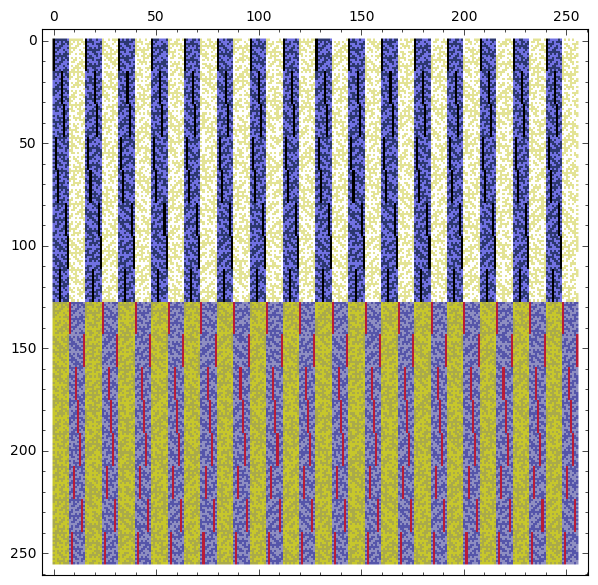
\includegraphics[width=.9\linewidth]{../matrix_plot/re8_10_bent_cayley_graph_index_matrix.png}
  \captionof{figure}{$[f_{8,10}]$: 10 extended Cayley classes ~~ ~~~~ ~~~~ ~~~~~~~~~}
  \label{fig:c8_10_bent_cayley_graph_index_matrix}
\end{minipage}
\begin{minipage}{.48\textwidth}
  \centering
  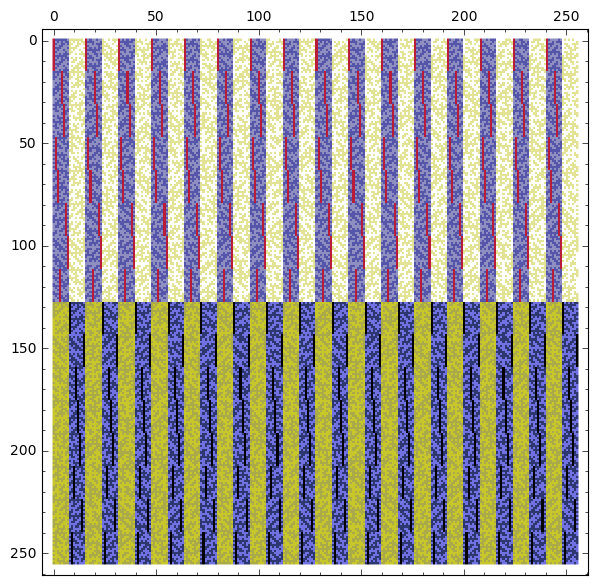
\includegraphics[width=.9\linewidth]{../matrix_plot/re8_10_dual_cayley_graph_index_matrix.png}
  \captionof{figure}{$[f_{8,10}]$: 10 extended Cayley classes of dual bent functions}
  \label{fig:c8_10_dual_cayley_graph_index_matrix}
\end{minipage}%
\end{figure}
6 of the 10 classes form 3 dual pairs of classes.
% \end{frame}
% \end{colortheme}
% \begin{colortheme}{seagull}
% \begin{frame}

\paragraph*{Partial spread bent functions.}

According to Langevin and Hou \cite{LanH11counting}
there are $70576747237594114392064 \approx 2^{75.9}$ \Emph{partial spread} bent functions in
dimension 8,
contained in $14758$ EA classes, of which $14756$ classes have degree 4.
%
%~
%
The EA class representatives are listed at Langevin's web site
%
\begin{verbatim}
http://langevin.univ-tln.fr/project/spread/psp.html
\end{verbatim}

%\slidecite{Langevin and Hou 2011}
% \end{frame}
% \end{colortheme}
% \begin{colortheme}{jubata}
% \begin{frame}
\paragraph*{Example partial spread ET class $[psf_{9,5439}]$.}
\begin{figure}[!hb]
\centering
\begin{minipage}{.48\textwidth}
  \centering
  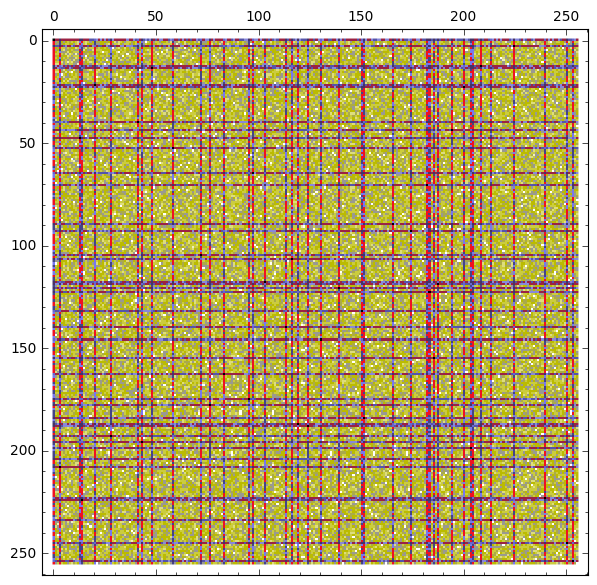
\includegraphics[width=.9\linewidth]{../matrix_plot/psf_9_5439_bent_cayley_graph_index_matrix.png}
  \captionof{figure}{$[psf_{9,5439}]$: 16 extended Cayley classes ~~ ~~~~ ~~~~ ~~~~~~~~~}
  \label{fig:psf_9_5439_bent_cayley_graph_index_matrix}
\end{minipage}
\begin{minipage}{.48\textwidth}
  \centering
  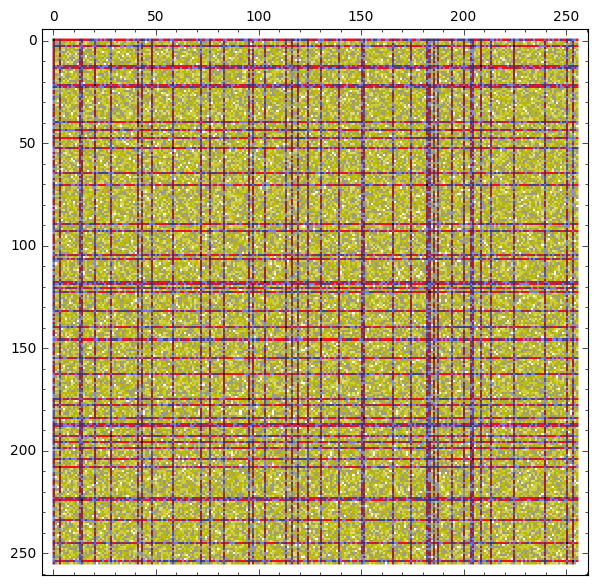
\includegraphics[width=.9\linewidth]{../matrix_plot/psf_9_5439_dual_cayley_graph_index_matrix.png}
  \captionof{figure}{$[psf_{9,5439}]$: 16 extended Cayley classes of dual bent functions}
  \label{fig:psf_9_5439_dual_cayley_graph_index_matrix}
\end{minipage}%
\end{figure}
6 of the 16 classes form 3 dual pairs of classes.
% \end{frame}

\section{SageMath and SageMathCloud code}
\label{sec-Code}
% \begin{frame}[fragile]
%\subsection{Public worksheet on SageMathCloud}
~

Bliss: \cite{JunK07Bliss,JukN11conflict}

Boolean-Cayley-graphs: GitHub repository \cite{Leo16GitHub} and SageMathCloud folder
\cite{Leo16SMC}.

Nauty: \cite{McKP13nauty,McKP14practical}

Coding theory and cryptography in Sage: \cite{JoyEtAl13Sage}

SageMath: \cite{SageMath7517}

SageMathCloud: \cite{SageMathCloud}.

% \end{frame}

\begin{itemize}
 \item 2015-04 to 2015-05 SageMathCloud: Cliques-Automorphisms project starts looking at Cayley
classes for bent functions of dimension up to 6, using BooleanFunction and \verb!is_isomorphic()!.
 \item 2015-12 SageMathCloud: Cliques-Automorphisms project
worksheets produced initial results used in the ACCMCC presentation.
The worksheets were too slow to effectively tackle bent functions in 8 dimensions.
 \item 2016-07 SageMath: Downloaded Sage and began refactoring worksheets into Sage code.
 \item 2016-08 GitHub: Uploaded refactored Sage code to new Boolean-Cayley-graphs project.
 \item 2016-08 SageMath: Began using canonical labels rather than directly testing for isomorphism
between Cayley graphs.
Canonical labelling uses the Bliss algorithm, speeding up computation in comparison to the default
Sage algorithm,
and allows comparison between graphs using equality of canonically labelled graphs rather than
isomorphism, also giving a speed boost.
This finally made it feasible to check bent functions in 8 dimensions up to degree 3.
 \item 2016-09 SageMath: Changed many Sage code files into Python modules.
Introduced a BentFunction class.
 \item 2016-11 SageMath: \verb!check_graphs_using_gap!
\end{itemize}


\section{Discussion}
\label{sec-Discussion}
% \begin{frame}
%\subsection{Questions (1)}
The following questions have been settled only for $m \leqslant 3$:
\begin{enumerate}
\item
How many EC classes are there for each $m$?
Are there ``Exponential numbers'' of classes \cite{Kan83exponential}?
\item
Are there any ET classes that contain the maximum number, $16^m$, different EC classes?
\item
Which EC classes overlap more than one ET class?
\item
Which bent functions are Cayley equivalent to their dual?
\end{enumerate}

Also, what are the remaining EA and EC classes for $m=4$,
i.e. the EA and EC classes of binary bent functions of dimension 8 and degree 4 \cite{LanL11counting}?

% \slidecite{Kantor 1983; Jungnickel and Tonchev 1991; Langevin and Leander 2008, 2011}
% \end{frame}

\appendix

\section{Proof of Theorem \ref{th-Quadratic-Classes}}
\label{app-proof-of}

The proof of Theorem \ref{th-Quadratic-Classes} relies on a number of supporting lemmas,
which are stated and proved here.
\begin{Lemma}
\label{lm-notes-5}
Let $q(x) := x^T L x$ where $L \in \Z_2^{2 m \times 2 m}$,
\begin{align*}
L
&:=
\left[
\begin{array}{cc}
0 & I
\\
0 & 0
\end{array}
\right],
\intertext{so that}
q(x) &= \sum_{k=0}^{m-1} x_k x_{m+k}.
\end{align*}

Let $f(x) := q(x+b) + \langle c,x \rangle + q(b)$.
Then there exists $c' \in \Z_2^{2m}$ such that
\begin{align*}
f(x)
&=
q(x) + \langle c',x \rangle.
\end{align*}

\end{Lemma}

\begin{proof}
\begin{align*}
q(x) = x^T L x, \quad \text{so~}
q(x+b)
&=
(x^T+b^T) L (x+b)
\\
&= q(x) + x^T L b + b^T L x + q(b)
\\
&= q(x) + \langle (L + L^T) b, x \rangle + q(b),
\intertext{and therefore}
q(x+b) + \langle c, x \rangle + q(b)
&=
q(x) + \langle (L+L^T) b + c, x \rangle.
\end{align*}

\end{proof}

\begin{Lemma}
\label{lm-notes-3}
Let $Z \in \Z_2^{2 m \times 2 m}$ be symmetric with zero diagonal.
In other words, $Z = Z^T$, $\diag{Z} = 0$.
Then for any $M \in \Z_2^{2 m \times 2 m}$,
\begin{align*}
x^T (M + Z) x  &= x^T M x
\end{align*}
for all $x \in \Z^{2 m}$.
\end{Lemma}

\begin{proof}
Let $Z$, $x$ be as above.
Then
\begin{align*}
x^T Z x
&=
\sum_{i=0}^{2m-1} \sum_{j=0}^{2m-1} x_i Z_{i,j} x_j
\\
&=
\sum_{i=0}^{2m-1} \sum_{j<i} x_i Z_{i,j} x_j +
\sum_{i=0}^{2m-1} x_i Z_{i,i} x_i +
\sum_{i=0}^{2m-1} \sum_{j>i} x_i Z_{i,j} x_j
\\
&=
\sum_{i=0}^{2m-1} \sum_{j<i} x_i (Z_{i,j} + Z_{j,i})
= 0.
\intertext{Therefore}
x^T (M + Z) x  &= x^T M x + x^T Z x = x^T M x.
\end{align*}
\end{proof}

\begin{Lemma}
\label{lm-notes-4}
Let $q$ be defined as per Lemma \ref{lm-notes-5}.
Then for all $c \in Z_2^{2 m}$ with $q(c)=0$, there exists $A \in GL(2 m, 2)$ such that
\begin{align*}
q(A x) &= q(x) + \langle c, x \rangle.
\end{align*}
\end{Lemma}

\begin{proof}
Let $C \in \Z_2^{2 m \times 2 m}$ be such that $C_{i,j} = \delta_{i,j} c_i$, where $\delta$ is the
\Emph{Dirac delta}: $\delta_{i,j}=1$ if $i=j$ and $0$ otherwise.
In other words $\diag{C} = c$.
Then
\begin{align*}
\langle c, x \rangle
&=
\sum_{i=0}^{2m-1} c_i x_i
\\
&=
\sum_{i=0}^{2m-1} x_i c_i x_i
=
x^T C x.
\end{align*}
Therefore, by Lemma \ref{lm-notes-3},
\begin{align*}
q(x) + \langle c, x \rangle
&=
x^T (L + Z + C) x,
\end{align*}
where $Z \in \Z_2^{2 m \times 2 m}$ is symmetric with zero diagonal.

For such $Z$, let $S := Z + C$.
We want to find $A \in \Z_2^{2 m \times 2 m}$ such that $q(A x) = q(x) + \langle c, x \rangle.$
In other words,
\begin{align*}
q(A x)
&=
(A x)^T L (A x)
=
x^T A^T L A x
=
x^T (L + S) x.
\end{align*}
This will be true if $A^T L A = L + S.$

Let
\begin{align*}
A
&:=
\left[
\begin{array}{cc}
A_{0,0} & A_{0,1}
\\
A_{1,0} & A_{1,1}
\end{array}
\right],
\quad
S
&:=
\left[
\begin{array}{cc}
S_{0,0} & S_{0,1}
\\
S_{0,1}^T & S_{1,1}
\end{array}
\right]
=:
\left[
\begin{array}{cc}
Z_{0,0} + C_{0,0} & Z_{0,1}
\\
Z_{0,1}^T & Z_{1,1} + C_{1,1}
\end{array}
\right].
\end{align*}
Since
\begin{align*}
L A
&=
\left[
\begin{array}{cc}
0 & I
\\
0 & 0
\end{array}
\right]
\left[
\begin{array}{cc}
A_{0,0} & A_{0,1}
\\
A_{1,0} & A_{1,1}
\end{array}
\right]
=
\left[
\begin{array}{cc}
A_{1,0} & A_{1,1}
\\
0 & 0
\end{array}
\right],
\end{align*}
we require that
\begin{align*}
A^T L A
&=
\left[
\begin{array}{cc}
A_{0,0} & A_{1,0}
\\
A_{0,1} & A_{1,1}
\end{array}
\right]
\left[
\begin{array}{cc}
A_{1,0} & A_{1,1}
\\
0 & 0
\end{array}
\right]
\\
&=
\left[
\begin{array}{cc}
A_{0,0}^T A_{1,0} & A_{0,0}^T A_{1,1}
\\
A_{0,1}^T A_{1,0} & A_{0,1}^T A_{1,1}
\end{array}
\right]
\\
&=
L + S
=
\left[
\begin{array}{cc}
S_{0,0} & I + S_{0,1}
\\
S_{0,1}^T & S_{1,1}
\end{array}
\right],
\end{align*}
and therefore
\begin{align*}
A_{0,0}^T A_{1,0}
&=
S_{0,0},
\quad
A_{0,0}^T A_{1,1}
=
I + S_{0,1},
\\
A_{0,1}^T A_{1,0}
&=
S_{0,1}^T,
\quad
A_{0,1}^T A_{1,1}
=
S_{1,1}.
\end{align*}
If $S_{0,1}=0$ and $A_{0,0}=I$ then
$A_{1,0}=S_{0,0}$, $A_{1,1}=I$ and $A_{0,1}=S_{1,1}$.
In this case, we have $A_{0,1}^T A_{1,0} = S_{0,1}^T = 0$,
i.e. $S_{1,1} S_{0,0} = 0$, and
\begin{align*}
A
&=
\left[
\begin{array}{cc}
I & S_{1,1}
\\
S_{0,0} & I
\end{array}
\right],
\intertext{so that}
A^T L A
&=
\left[
\begin{array}{cc}
I & S_{0,0}
\\
S_{1,1} & I
\end{array}
\right]
\left[
\begin{array}{cc}
S_{0,0} & I
\\
0 & 0
\end{array}
\right]
\\
&=
\left[
\begin{array}{cc}
S_{0,0} & I
\\
0 & S_{1,1}
\end{array}
\right]
\\
&=
L + S.
\end{align*}

Also
\begin{align*}
S
&=
\left[
\begin{array}{cc}
Z_{0,0} + C_{0,0} & 0
\\
0 & Z_{1,1} + C_{1,1}
\end{array}
\right].
\end{align*}

Since $q(c)=0$ we have
\begin{align*}
q(c)
&=
\sum_{k=0}^{m-1} c_k c_{m+k}
=
0.
\end{align*}
Let $K := \{ k \mid c_k c_{m+k} = 1 \}$.
Then we must have $\abs{K} = 2 r$ for some integer $r \geqslant 0$, i.e. $\abs{K}$ is even.
We therefore arbitrarily group the elements of $K$ into pairs $(i_p, j_p)$ for $p=0,\ldots,r-1$,
and define the matrix $T \in \Z_2^{m \times m}$ by
\begin{align*}
T_{i,j}
&:=
\sum_{p=0}^{r-1} (\delta_{i,i_p} \delta_{j,j_p} + \delta_{i,j_p} \delta_{j,i_p}),
\end{align*}
so that
\begin{align*}
\begin{cases}
T_{i_p,j_p}
=
T_{j_p,i_p}
=
1
&\text{for~} p \in \{0,\ldots,r-1\},
\\
T_{i,j} = 0
&\text{otherwise.}
\end{cases}
\end{align*}
Since the $r$ pairs $(i_p, j_p)$ partition the set $K$,
the matrix $T$ has at most one non-zero in each row and column.

Recalling that
\begin{align*}
(T^2)_{i,j}
&=
\sum_{k=0}^{m-1} T_{i,k} T_{k,j},
\end{align*}
we see that the general term $T_{i,k} T_{k,j}$ of this sum is non-zero only if either
\begin{align*}
\begin{cases}
i = j = i_p,&\text{and}\ k=j_p,\ \text{or}
\\
i = j = j_p,&\text{and}\ k=i_p,
\end{cases}
\end{align*}
for some $p \in \{0,\ldots,r-1\}$, with all $2r$ of these cases being mutually exclusive.
So $T^2$ is diagonal with $2r$ non-zeros at the elements of $K$.

But $C_{1,1} C_{0,0}$ is diagonal, and $(C_{1,1} C_{0,0})_{i,i} = c_{m+i} c_i$.
Therefore
\begin{align}
T^2 &= C_{1,1} C_{0,0}.
\label{eq-t-2}
\end{align}

Now, let $Z_{0,0}=Z_{1,1}=T$. Then $S_{0,0} = T + C_{0,0}$, $S_{1,1} = T + C_{1,1}$, and
\begin{align*}
S_{1,1} S_{0,0}
&=
(T + C_{1,1})(T + C_{0,0})
=
T^2 + T C_{0,0} + C_{1,1} T + C_{1,1} C_{0,0}
\\
&=
T C_{0,0} + C_{1,1} T,
\end{align*}
where in the last step, we have used \eqref{eq-t-2}.

Now,
\begin{align*}
(T C_{0,0} + C_{1,1} T)_{i,j}
&=
\sum_{k=0}^{m-1} T_{i,k} (C_{0,0})_{k,j} + (C_{1,1})_{i,k} T_{k,j}
\\
&=
T_{i,j} (C_{0,0})_{j,j} + (C_{1,1})_{i,i} T_{i,j}
\\
&=
T_{i,j} \left( c_j + c_{m+i} \right).
\end{align*}
As above, $T_{i,j}$ is non-zero only when $(i,j)=(i_p,j_p)$ or $(i,j)=(j_p,i_p)$
for some $p \in \{0,\ldots,r-1\}$, but in all those cases $c_j=c_{m+j}=1$.

Therefore
\begin{align*}
S_{1,1} S_{0,0} &= T C_{0,0} + C_{1,1} T = 0.
\end{align*}
Similarly, $S_{0,0} S_{1,1} = 0$, and therefore
\begin{align*}
A^2
&=
\left[
\begin{array}{cc}
I & S_{1,1}
\\
S_{0,0} & I
\end{array}
\right]
\left[
\begin{array}{cc}
I & S_{1,1}
\\
S_{0,0} & I
\end{array}
\right]
\\
&=
\left[
\begin{array}{cc}
I + S_{1,1} S_{0,0} & S_{1,1} + S_{1,1}
\\
S_{0,0} + S_{0,0} & I + S_{0,0} S_{1,1}
\end{array}
\right]
=
\left[
\begin{array}{cc}
I & 0
\\
0 & I
\end{array}
\right].
\end{align*}

We have therefore shown that
\begin{align}
A
&:=
\left[
\begin{array}{cc}
I & T + C_{1,1}
\\
T + C_{0,0} & I
\end{array}
\right],
\quad
S
:=
\left[
\begin{array}{cc}
T + C_{0,0} & 0
\\
0 & T + C_{1,1}
\end{array}
\right]
\label{eq-a-s-def}
\end{align}
is a solution to $A^T L A = L + S$ with $A \in GL(2 m, 2)$.

Finally, given $c$ with $q(c)=0$, the matrix $A$ as defined by \eqref{eq-a-s-def} is such that
$q(A x) = q(x) + \langle c, x \rangle$.
\end{proof}
% \end{frame}

\begin{Lemma}
\label{lm-notes-6}
For $k \in \{0,\ldots,m-1\}$ define $e^{(k)}$ by
\begin{align}
e_i^{(k)} &:= \delta_{i,k} + \delta_{i,m+k}
\label{eq-e-def}
\end{align}
for $i \in \{0,\ldots,2 m - 1\}$.

Let $h(x) := q(x) + \langle e^{(0)}, x \rangle$, where $q$ is defined as per Lemma \ref{lm-notes-5}.
Then for any $c'$ such that $q(c')=1$, there exists $B \in GL(2 m, 2)$ such that
\begin{align}
h(B x) &= q(x) + \langle c',x \rangle.
\label{eq-h-B-x}
\end{align}
\end{Lemma}

\begin{proof}
Let $K'=\{k \mid c'_k c'_{m+k} = 1\}$. Since $q(c')=1$, $\abs{K'}$ is odd.
Choose any $\ell \in K'$, and let $c := c' + e^{(\ell)}$.
Then $c_{\ell} = c_{m+\ell} = 0$ and $q(c)=0$.

Now let $h^{(\ell)}(x) := q(x) + \langle e^{(\ell)}, x \rangle$.
We calculate
\begin{align*}
h^{(\ell)}(A x)
&=
q(A x) + \langle e^{(\ell)}, A x \rangle
=
q(x) + \langle c, x \rangle + \langle A^T e^{(\ell)}, x \rangle
\\
&=
q(x) + \langle c + A^T e^{(\ell)}, x \rangle
\end{align*}
for $A$ given by the proof of Lemma \ref{lm-notes-4}.

If we let $K := \{ k \mid c_k c_{m+k} = 1 \}$, we see that $K = K' \setminus \{\ell\}$.
Applying the other definitions and techniques used in the proof of Lemma \ref{lm-notes-4},
we see that since $c_{\ell} = c_{m+\ell} = 0$ and $K$ does not contain $\ell$,
column $\ell$ of each of $S_{0,0} := T + C_{0,0}$
and $S_{1,1} := T + C_{1,1}$ is $0$, and therefore columns $\ell$ and $m + \ell$ of
\begin{align*}
A^T + I
&:=
\left[
\begin{array}{cc}
I & T + C_{0,0}
\\
T + C_{1,1} & I
\end{array}
\right]
\end{align*}
are both $0$.
Therefore $A^T e^{(\ell)} = e^{(\ell)}$, and therefore
\begin{align*}
h^{(\ell)}(A x)
&=
q(x) + \langle c', x \rangle.
\end{align*}

\end{proof}

\begin{Lemma}
\label{lm-notes-6-b}
For distinct $k,\ell \in \{0,\ldots,m-1\}$ let $e^{(k)}, e^{(\ell)}$ be defined as per Lemma
\ref{lm-notes-6}.
Let $h(x) := q(x) + \langle e^{(k)}, x \rangle$, where $q$ is defined as per Lemma \ref{lm-notes-5}.
Then there exists $A \in GL(2 m, 2)$ such that
\begin{align}
h(A x)
&=
q(x) + \langle e^{(\ell)},x \rangle.
\end{align}
\end{Lemma}

\begin{proof}
The matrix $A$ is the permutation matrix for the the permutation $(k\ \ell)(m+k\ m+\ell)$ (defined
using cycle notation.)
\end{proof}

\begin{Lemma}
\label{lm-notes-7}
Let $q$ be defined as per Lemma \ref{lm-notes-5}.
Then for all $c, c' \in Z_2^{2 m}$ with $q(c)=q(c')=1$, there exists $A \in GL(2 m, 2)$ such that
if $h(x) := q(x) + \langle c, x \rangle$, then
\begin{align*}
h(A x) &= q(x) + \langle c', x \rangle.
\end{align*}
\end{Lemma}

\begin{proof}
This is a consequence of Lemmas \ref{lm-notes-6} and \ref{lm-notes-6-b}.
\end{proof}

\begin{proofof}{Theorem \ref{th-Quadratic-Classes}}
It is well known that all quadratic bent functions are contained in one Extended Affine equivalence
class.
As a consequence of Theorem \ref{th-Affine-Translate-Cayley}, without loss of generality, we need
only examine
the Extended Translation equivalence class of the quadratic function $q$ as defined in Lemma
\ref{lm-notes-5}.

As a result of Lemma \ref{lm-notes-5}, we actually need only examine functions of the form
$f(x) = q(x) + \langle c,x \rangle$
for some $c \in \Z_2^{2m}$.
Lemma \ref{lm-notes-4} implies that all such functions for which $q(c)=0$ are Cayley equivalent to
$q$.
Lemma \ref{lm-notes-7} implies that any two such functions $q(x) + \langle c, x \rangle$ and $q(x) +
\langle c', x \rangle$
with $q(c)=q(c')=1$ are Cayley equivalent to each other.

The functions where $q(c)=0$ are not Cayley equivalent to the functions where $q(c)=1$ because
Lemma \ref{lm-notes-9b} implies that
\begin{align*}
\weightclass{x \mapsto q(x) + \langle c,x \rangle}
&=
\dual{q}(c) = q(c),
\end{align*}
since $q$ is self-dual.
\end{proofof}

%%%%%%%%%%%%%%%%%%%%%%%%%%%%%%%%%%%%%%%%%%%%%%%%%%%%%%%%%%%%%%
\paragraph*{Acknowledgements.}

Thanks to Christine Leopardi for her hospitality at Long Beach.
Thanks to Robert Craigen, Joanne Hall, William Martin,
Padraig {\'O} Cath{\'a}in and Judy-anne Osborn for valuable discussions.
This work was begun in 2014 while the author was a Visiting Fellow at the Australian National University,
and concluded while the author was a Visiting Fellow and a Casual Academic at the University of Newcastle, Australia.
%Thanks also to the anonymous reviewer of the previous draft of this paper.

%%%%%%%%%%%%%%%%%%%%%%%%%%%%%%%%%%%%%%%%%%%%%%%%%%%%%%%%%%%%%%%%%%%%%%

%\addtocontents{toc}{\vspace{0.5cm}}

%\newpage

\bibliographystyle{abbrv-par}

\bibliography{bib}

%\input{AJC-2015-Leopardi-Twin-bent-Hurwitz-Radon-revised.bbl}

\end{document}
% ----------------------------------------------------------------
